\documentclass[a4paper,12pt, oneside]{book}

% \usepackage{fullpage}
\usepackage[italian]{babel}
\usepackage[utf8]{inputenc}
\usepackage{amssymb}
\usepackage{amsthm}
\usepackage{graphics}
\usepackage{amsfonts}
\usepackage{listings}
\usepackage{amsmath}
\usepackage{amstext}
\usepackage{engrec}
\usepackage{rotating}
\usepackage{verbatim}
\usepackage[safe,extra]{tipa}
%\usepackage{showkeys}
\usepackage{multirow}
\usepackage{hyperref}
\usepackage{microtype}
\usepackage{fontspec}
\usepackage{enumerate}
\usepackage{braket}
\usepackage{marginnote}
\usepackage{pgfplots}
\usepackage{cancel}
\usepackage{polynom}
\usepackage{booktabs}
\usepackage{enumitem}
\usepackage{framed}
\usepackage{pdfpages}
\usepackage{pgfplots}
\usepackage{algorithm}
% \usepackage{algpseudocode}
\usepackage[cache=false]{minted}
\usepackage{mathtools}
\usepackage[noend]{algpseudocode}

\usepackage{tikz}\usetikzlibrary{er}\tikzset{multi  attribute /.style={attribute
    ,double  distance =1.5pt}}\tikzset{derived  attribute /.style={attribute
    ,dashed}}\tikzset{total /.style={double  distance =1.5pt}}\tikzset{every
  entity /.style={draw=orange , fill=orange!20}}\tikzset{every  attribute
  /.style={draw=MediumPurple1, fill=MediumPurple1!20}}\tikzset{every
  relationship /.style={draw=Chartreuse2,
    fill=Chartreuse2!20}}\newcommand{\key}[1]{\underline{#1}}
  \usetikzlibrary{arrows.meta}
  \usetikzlibrary{decorations.markings}
  \usetikzlibrary{arrows,shapes,backgrounds,petri}
\tikzset{
  place/.style={
        circle,
        thick,
        draw=black,
        minimum size=6mm,
    },
  transition/.style={
    rectangle,
    thick,
    fill=black,
    minimum width=8mm,
    inner ysep=2pt
  },
  transitionv/.style={
    rectangle,
    thick,
    fill=black,
    minimum height=8mm,
    inner xsep=2pt
    }
  } 
\usetikzlibrary{automata,positioning}
\usepackage{fancyhdr}
\pagestyle{fancy}
\fancyhead[LE,RO]{\slshape \rightmark}
\fancyhead[LO,RE]{\slshape \leftmark}
\fancyfoot[C]{\thepage}


\title{Processo e Sviluppo del Software}
\author{UniShare\\\\Davide Cozzi\\\href{https://t.me/dlcgold}{@dlcgold}}
\date{}

\pgfplotsset{compat=1.13}
\begin{document}
\maketitle

\definecolor{shadecolor}{gray}{0.80}
\setlist{leftmargin = 2cm}
\newtheorem{teorema}{Teorema}
\newtheorem{definizione}{Definizione}
\newtheorem{esempio}{Esempio}
\newtheorem{corollario}{Corollario}
\newtheorem{lemma}{Lemma}
\newtheorem{osservazione}{Osservazione}
\newtheorem{nota}{Nota}
\newtheorem{esercizio}{Esercizio}
\algdef{SE}[DOWHILE]{Do}{doWhile}{\algorithmicdo}[1]{\algorithmicwhile\ #1}
\tableofcontents
\renewcommand{\chaptermark}[1]{%
  \markboth{\chaptername
    \ \thechapter.\ #1}{}}
\renewcommand{\sectionmark}[1]{\markright{\thesection.\ #1}}
\newcommand{\floor}[1]{\lfloor #1 \rfloor}
\newcommand{\MYhref}[3][blue]{\href{#2}{\color{#1}{#3}}}%
\chapter{Introduzione}
\textbf{Questi appunti sono presi a lezione. Per quanto sia stata fatta
  una revisione è altamente probabile (praticamente certo) che possano
  contenere errori, sia di stampa che di vero e proprio contenuto. Per
  eventuali proposte di correzione effettuare una pull request. Link: }
\url{https://github.com/dlcgold/Appunti}.\\
\textbf{Le immagini presenti in questi appunti sono tratte dalle slides del
  corso e tutti i diritti delle stesse sono da destinarsi ai docenti del corso
  stesso}.
\chapter{Metodi Agili}
I \textit{metodi agili} sono stati definiti per rispondere all'esigenza di dover
affrontare lo sviluppo di software in continuo cambiamento. Durante lo sviluppo
si hanno vari passaggi:
\begin{itemize}
  \item comprensione dei prerequisiti
  \item scoperta di nuovi requisiti o cambiamento dei vecchi
\end{itemize}
Questa situazione rendeva difficile lo sviluppo secondo il vecchio metodo
\textit{waterfall} (a cascata) portando al fallimento di diversi progetti.\\
I \textit{metodi agili} ammettono che i requisiti cambino in modo ``naturale''
durante il processo di sviluppo software e per questo assumono un modello di
processo \textit{circolare}, con iterazioni della durata di un paio di settimane
(figura \ref{agile}). Potenzialmente dopo un'iterazione si può arrivare ad un
prodotto che può essere messo ``in produzione''. Dopo ogni rilascio si
raccolgono \textit{feedback} per poter rivalutare i requisiti e migliorare il
progetto.\\
\begin{figure}
  \centering
  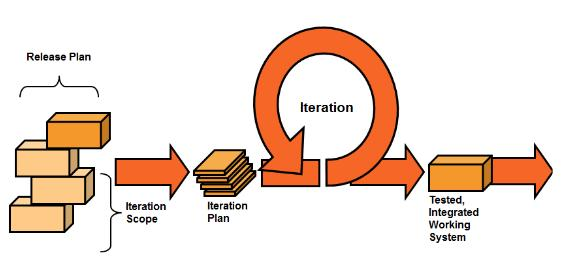
\includegraphics[scale = 0.6]{img/agile.jpg}
  \caption{Rappresentazione grafica del modello agile. I blocchi a sinistra
    rappresentano i requisiti (da sviluppare secondo una certa priorità). Lo
    sviluppo si articola tramite varie iterazioni che porta ogni volta ad
    aggiungere una parte al prodotto finale (ogni iterazione produce, a partire
    da un certo requisito, un parte di
    prodotto di qualità già definitiva, con testing, documentazione
    etc$\ldots$)}
  \label{agile}
\end{figure}
Si hanno quindi aspetti comuni nei metodi agili e nel loro processo:
\begin{itemize}
  \item enfasi sul team, sulla sua qualità e sulla sua selezione
  \item il team è \textit{self organizing}, si da importanza ai vari membri del
  team dato che non esiste un \textit{manager} ma
  è il team stesso a gestire lo sviluppo
  \item enfasi al pragmatismo, focalizzandosi su una documentazione
  efficace evitando di produrre documenti inutili e difficili da mantenere
  \item enfasi sulla comunicazione diretta, sostituendo i documenti suddetti con 
  meeting e riunioni periodiche
  \item enfasi sull'idea che nulla sia definitivo: la perfezione non deve essere 
  seguita fin da subito ma saranno gli step a portare al
  raggiungimento di una perfezione finale (anche dal punto di vista del design)
  \item enfasi sul controllo costante della qualità del prodotto, anche tramite
    \begin{itemize}
      \item \textit{continuous testing} grazie al quale un insieme
  di test viene eseguito in modo automatico dopo ogni modifica
      \item \textit{analisi statica e dinamica} del codice al fine di trovare difetti
  nello stesso
      \item \textit{refactoring}
    \end{itemize}

\end{itemize}
I metodi agili sono molto ``elastici'' e permettono la facile
  definizione di nuovi metodi facilmente adattabili al singolo progetto.
\section{Scrum}
Uno dei più famosi, tra i vari \textit{metodi agili}, è \textbf{scrum} (figura
\ref{scrum}).\\
In questo caso la parte di sviluppo e iterazione prende il nome di
\textit{sprint} ed ha una durata variabile tra una e quattro settimane, per avere
un rilascio frequente e una veloce raccolta di feedback. I requisiti sono
raccolti nel cosiddetto \textit{product backlog}, con priorità basata sulla base
delle indicazioni del committente. Ad ogni \textit{sprint} si estrae dal
\textit{product backlog} lo \textit{sprint backlog}, ovvero il requisito (o i
requisiti) da implementare nello \textit{sprint}. Lo \textit{sprint backlog}
viene analizzato nel dettaglio producendo i vari \textit{backlog items}, ovvero
le singole funzionalità che verranno implementate nello \textit{sprint}. Si
ottiene quindi di volta in volta un pezzo di prodotto finale, testato e
documentato. Durante le settimane di \textit{sprint} si effettua anche un meeting
giornaliero utile per mantenere alti i livelli di comunicazione e visibilità
dello sviluppo. Durante il meeting ogni sviluppatore risponde a tre domande:
\begin{enumerate}
  \item Cosa è stato fatto dall'ultimo meeting?
  \item Cosa farai fino al prossimo meeting?
  \item Quali sono le difficoltà incontrate?
\end{enumerate}
L'ultimo punto permette la cooperazione tra \textit{team members}, consci di cosa
ciascuno stia facendo.\\
\begin{figure}
  \centering
  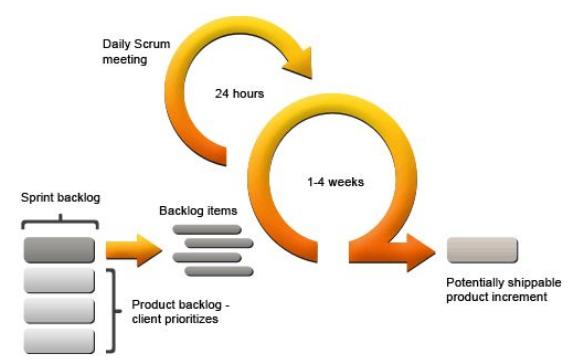
\includegraphics[scale = 0.6]{img/scrum.jpg}
  \caption{Rappresentazione grafica del processo scrum}
  \label{scrum}
\end{figure}
Durante il processo \textit{scrum} si hanno quindi tre ruoli:
\begin{enumerate}
  \item il \textbf{product owner}, il committente che partecipa tramite feedback
  e definizione dei requisiti
  \item il \textbf{team} che sviluppa
  \item lo \textbf{scrum master} che controlla la correttezza di svolgimento del processo scrum 
\end{enumerate}
Essi collaborano nelle varie fasi:
\begin{itemize}
  \item product owner e team collaborano nella definzione dei backlog e nella
  loro selezione ad inizio \textit{sprint}
  \item durante lo \textit{sprint} lavora solo il team
  \item nello studio del risultato collaborano tutti coloro che hanno un
  interesse diretto nel progetto (team, product owner e stakeholders) 
\end{itemize}
\textit{Lo scrum master interagisce in ogni fase, fase che viene comunque
  guidata tramite meeting}:
\begin{itemize}
  \item \textbf{sprint planning meeting}, ad inizio \textit{sprint}
  \item \textbf{daily scrum meeting}, il meeting giornaliero
  \item \textbf{sprint review meeting}, in uscita dallo \textit{sprint} per lo
  studio dei risultati
  \item \textbf{sprint retrospective meeting}, in uscita dallo \textit{sprint}
  per lo studio tra i membri del team di eventuali migliorie al processo e allo
  sviluppo del prodotto (anche dal punto di vista delle tecniche e delle
  tecnologie)
\end{itemize}
\section{Extreme Programming}
Un altro tipo di metodo agile è l'\textit{extreme programming} (figura
\ref{extreme}), ormai poco usato. I requisiti prendono i nomi di
\textit{stories}, delle narrazioni in cui l'attore (futuro utente del sistema) cerca 
di svolgere un compito. Vengono
scelti quindi \textit{stories} per la prossima iterazione, dove si hanno testing
e revisione continua. Le release di ogni iterazione vengono catalogate per
importanza (con anche la solita collezione di feedback). In \textit{extreme
  programming} si hanno davvero molte pratiche:
\begin{itemize}
  \item The Planning Game
  \item Short Releases
  \item Metaphor
  \item Simple Design
  \item Refactoring
  \item Test-First Design
  \item Pair Programming
  \item Collective Ownership (codice condiviso da tutti senza alcun owner, con
  tutti in grado di effettuare modifiche)
  \item Continuous Integration
  \item 40-Hour Week
  \item On-Site Customer
  \item Coding Standard (per avere il collective ownership avendo un solo
  standard di codifica comune a tutti)
  \item Open workspace
\end{itemize}
\begin{figure}
  \centering
  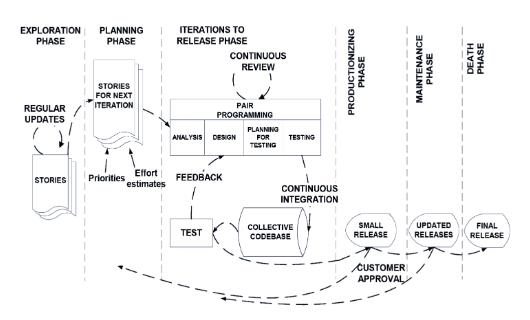
\includegraphics[scale = 0.7]{img/extreme.jpg}
  \caption{Rappresentazione grafica dell'extreme programming}
  \label{extreme}
\end{figure}
\chapter{DevOps}
Nel tempo si è passato dal \textit{modello waterfall} (dove tutto era definito
ad inizio progetto) al \textit{modello agile}. Negli ultimi tempi si è
sviluppato un altro metodo, chiamato \textbf{DevOps}, dove anche la parte di
\textit{operation} deve essere agile: il rilascio in produzione e il
\textit{deployment} devono essere agili quanto lo sviluppo. Amazon, Netflix,
Facebook e molte altre società già adottano le pratiche \textit{DevOps.}\\
Nel \textit{DevOps} i team di sviluppo e operation sono indipendenti tra loro,
diminuendo il costo di impegno necessario al team di sviluppo per la parte di
deployment (che viene resa anche più sicura grazie alla diminuzione
dell'intervento umano in favore di automazioni). Inoltre, avendo i due team dei
tempi di lavoro diversi, si riesce a prevenire ritardi causati dalla non
organicità delle operazioni.\\
DevOps promuove la collaborazione tra di due team al fine di ottenere una sorta
di team unico che curi sia sviluppo che operation.\\
DevOps include quindi diversi processi che vengono automatizzati:
\begin{itemize}
  \item Continuous Development
  \item Continuous Integration
  \item Continuous Testing
  \item Continuous Deployment (anche con tecnologie di virtualizzazione e
  con l'uso di \textit{container} in \textit{ambiente cloud})
  \item Continuous Monitoring
\end{itemize}
Con DevOps il feedback arriva in primis dal software (i tool di
\textit{monitor}) inoltre il focus viene spostato sui processi automatici.\\
Nel DevOps si introducono nuovi ruoli:
\begin{itemize}
  \item il \textbf{DevOps Evangelist}, simile allo \textit{scrum master},
  supervisiona l'intero processo di DevOps
  \item l'\textbf{automation expert}, dedicato a curare gli aspetti di
  automatismo 
  \item un \textbf{Security Engineer}
  \item un \textbf{Software Developer}, nonché \textbf{Tester}
  \item un \textbf{Quality Assurance} che verifica la qualità del prodotto
  rispetto ai requisiti
  \item un \textbf{Code Release Manager} che si occupa sull'infrastruttura e
  sul deploy della release
\end{itemize}
Il DevOps (figura \ref{devops}) si basa su sei principi base:
\begin{enumerate}
  \item \textbf{Customer-Centric Action}, ovvero il committente è al centro
  dell'azione 
  \item \textbf{End-To-End Responsibility}, ovvero il team gestisce interamente
  il prodotto, avendone responsabilità totale
  \item \textbf{Continuous Improvement}, ovvero cercare continuamente di
  migliorare senza sprechi il prodotto finale e i servizi
  \item \textbf{Automate everything}, ovvero cercare di automatizzare l'intera
  infrastruttura di processo, dalle attività di testing e integrazione fino ad
  arrivare alla costruzione della release e del deployment
  \item \textbf{Work as one team}, ovvero unificare tutti gli aspetti sotto un
  unico team o comunque con due team che collaborano fortemente come se fossero
  uno 
  \item \textbf{Monitor and test everything}, ovvero testare e monitorare
  costantemente il prodotto
\end{enumerate}
\textit{Il quarto e il sesto punto sono i due punti tecnici principali}.
\begin{figure}
  \centering
  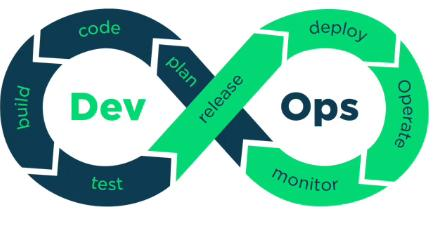
\includegraphics[scale = 0.6]{img/devops.jpg}
  \caption{Rappresentazione famosa del \textit{lifecycle} di DevOps, con le due
    parti, con le relative parti fondamentali, di sviluppo e operation distinte
    dai colori ma unite in un singolo metodo unico}
  \label{devops}
\end{figure}
\section{Build, Test e Release}
Partiamo dalla parte ``dev'' di DevOps.\\
Bisogna pensare a questi step in ottica di automatismo vicina al DevOps. \\
Innanzitutto bisogna introdurre i sistemi di \textbf{version control}, in primis
\textbf{Git}, un sistema di version control \textbf{distribuito}, dove ogni
utente ha una copia della repository (con la storia dei cambiamenti), con la
quale interagisce tramite \textit{commit} e \textit{update}. Esiste poi una
repository lato server per permettere di condividere i vari cambiamenti tramite
sincronizzazione.\\
\textbf{Git} permette anche lo sviluppo \textit{multi-branch} per permettere di
lavorare su più branch, pensando allo sviluppo separato dove ogni branch alla
fine può essere unito (\textit{merge}) con quello principale (solitamente
chiamato \textit{master}). Un altro branch standard è quello di sviluppo, detto
\textit{develop}. Un altro ancora è quello detto \textit{hotfix}, per le
modifiche più urgenti, che vive in uno stadio intermedio tra i due
sopracitati, prima ancora del branch \textit{develop}. Volendo ciascuna feature
può essere creata in un branch dedicato. Si procede con le versioni
``merge-ndo'' quando necessario, ``step by step'' fino ad un branch
\textit{release} per poi andare dopo il testing su \textit{master}. Sul branch
\textit{release} possono essere effettuati fix che poi verranno riportati anche
in \textit{develop}.\\
Lo sviluppo su multi-branch si collega alle operazioni di verifica che possono
essere attivate automaticamente a seconda dell'evoluzione del codice su ogni
branch. Avendo ogni branch una precisa semantica possiamo definire precise
attività di verifica, corrispondenti a \textit{pipelines} precise, solitamente
innescate da un \textit{push} di codice su un certo branch, in modo sia
automatico che manuale. Le pipeline vengono attivate in fase di test di un
componente, in fase di creazione di un sottosistema, di assembramento di un
sistema intero o di deployment in produzione. Si hanno quindi quattro fasi:
\begin{enumerate}
  \item component phase
  \item subsystem phase
  \item system phase
  \item production phase
\end{enumerate}
Spesso le pipelines sono usate
come \textit{quality gates} per valutare se un push può essere accettato in un
certo branch. Una pipeline può essere anche regolata temporalmente, in modo che
avvenga solo ad un certo momento della giornata.
\subsubsection{Component phase e Subsystem phase}
Dove il fuoco è sulla più piccola unità testabile che viene aggiornata (una
classe, un metodo etc$\ldots$) che non può essere eseguita senza l'intero
sistema. In tal caso si può fare:
\begin{itemize}
  \item code review
  \item unit testing
  \item static code analysis
\end{itemize}
Un cambiamento può anche essere testato nell'ambito del sottosistema di cui fa
parte, in tal caso si hanno anche check di prestazioni e sicurezza. Il servizio
però potrebbe essere da testare in isolamento rispetto ad altri servizi, usando
quindi dei \textit{mocks} o degli \textit{stubs}, ovvero creando degli alter ego
dei servizi mancanti in modo che il servizio da testare possa funzionare.
\subsubsection{System phase}
In questo caso si testa l'intero sistema che viene ``deployato'' in ambiente di
test. Si hanno:
\begin{itemize}
  \item integration tests
  \item performance tests
  \item security tests
\end{itemize}
Tutti test che richiedono l'interezza del sistema e sono spesso molto
dispendiosi e quindi bisogna regolare la frequenza di tali test in molti casi
(sfruttando ad esempio la notte).
\subsubsection{Production phase}
Questa fase è legata alla necessità di creare gli artefatti che andranno
direttamente ``sul campo'', ovvero il deployment in produzione. In tale fase
potrebbe essere necessario creare container o macchine virtuali. Si
hanno dei check molto veloci sugli artefatti finali (che non siano per esempio
corretti), dando per assodato che la qualità del codice sia già stata
testata. Si hanno quindi strategie anche di \textit{deployment incrementale},
per cui esistono più versioni del software contemporaneamente con diversa
accessibilità per gli utenti finali (accessibilità che viene man mano
scalata). In tal caso si usano anche vari tool di monitor. Si hanno anche
eventualmente tecniche di \textit{zero downtime} (dove il software non è mai in
uno stato \textit{unstable}).\\
\\
\textbf{Fasi diverse corrispondono a branch diversi}
\section{Deploy, Operate e Monitor}
Studiamo ora la parte ``Ops'' di DevOps.\\
Si studia l'evoluzione automatica del software da una versione all'altra in
produzione. Avanzare di versione in modo \textit{naive} e istantaneo è troppo
rischioso (qualora la nuova versione fosse corrotta non si avrebbe controllo
sull'update) e quindi spesso non attuabile (spesso anche per ragioni tecniche).
Si ha quindi un insieme di tecniche che si basano in primis
sull'\textit{evoluzione incrementale}. Tali tecniche si distinguono in base alla
dimensione su cui sono incrementati:
\begin{itemize}
  \item \textbf{Incremental wrt users:} \textit{Dark launching, Canary releases
    (and User Experimentation)}, ovvero legata agli utenti esposti alla nuova
  release
  \item \textbf{Incremental wrt requests:} \textit{Gradual upgrades/rollout},
  ovvero legata alle richieste per la nuova release
  \item \textbf{Incremental wrt components/replicas:} \textit{Rolling upgrade},
  incentrata sulle componenti che vengono aggiornate
  \item \textbf{Non-incremental with backups:} \textit{Green/blue deployment,
    Rainbow deployment}, non incrementali ma che offrono comunque un backup di
  sicurezza  
\end{itemize}
Tali schemi possono essere usati in un contesto DevOps.\\
Per studiare la prima tipologia (\textit{Incremental wrt users}) abbiamo:
\begin{itemize}
  \item \textbf{Dark launching} che arriva
  dal mondo di Facebook dal 2011. In tale schema 
  l'update è esposto solo ad una parte della popolazione, per la quale viene
  effettuato il deployment per studiare gli effetti (tramite continuous
  monitoring) ed eventuali modifiche e migliorie al software, che infine verrà
  deployato per il resto della popolazione in modo comunque incrementale fino a
  che l'intera popolazione godrà della feature. Spesso usata per front-end 
  \item \textbf{Canary releases}, che studia l'impatto di update relativi al
  back-end
\end{itemize}
Tali schemi spesso sono usati di pari passo per le varie sezioni del software,
nonché possono essere usati in modo intercambiabile.\\
Collegato a questi schemi si ha l'approccio basato sull'\textbf{user
  experimentation}, che non è un reale schema di gestione dell'evoluzione del
software ma è comunque correlato agli schemi sopra descritti. In questo
approccio si studiano diverse varianti del sistema e il loro impatto esponendole
agli utenti (perlomeno ad una sottoparte degli stessi in modo incrementale),
cercando di capire per l'utente cosa sia meglio e come (si ispira 
alla \textit{sperimentazione scientifico}). Si hanno quindi più release diverse,
per parti di popolazione comparabili, tra le quali si sceglierà la migliore.\\
Per la seconda tipologia (\textit{Incremental wrt requests}) si ha una divisione
a seconda delle richieste fatte dagli utenti (esempio un momento d'uso diverso
porta all'uso di componenti diverse), detto \textit{gradual rollout}. Si ha
quindi un \textit{load balancer} che 
permette la coesistenza di due versioni, una nuova e una vecchia, dello stesso
servizio. In modo graduale, partendo da pochissime, si passano le richieste alla
versione nuova per poter studiare e testare la nuova versione (in caso di
problemi il load balancer dirotterà tutte le richieste alla vecchia
versione). Alla fine tutto il traffico sarà diretto verso la nuova versione,
mentre la vecchia verrà dismessa.\\
Per la terza tipologia (\textit{Incremental wrt components/replicas}), si ha lo
schema del \textit{rolling upgrade}, dove l'upgrade non riguarda un singolo
upgrade ma tanti componenti di un sistema distribuito, verificando efficacia
di ogni singolo update tramite il continuous monitoring prima di effettuare
l'upgrade di un'altra componente. La stessa idea su applica anche a diverse
versioni dello stesso prodotto, aggiornandone una prima e poi le altre
progressivamente. Le nuove versioni delle componenti ``upgradate'' devono essere
compatibili con quelle ancora prive di upgrade.\\
Per la quarta tipologia (\textit{Non-incremental with backups}) si ha il
\textbf{blue/green deployment}, dove vengono isolate due copie della stessa
infrastruttura (anche hardware), dove una ospita la versione nuove l'altra la
vecchia. Un router ridireziona le richieste degli utenti verso le due unità e
quella che ospita la nuova 
versione subirà le solite operazioni di test che, se superate, porteranno il
router a direzionare verso quella unità, ignorando la vecchia. Se ci sono
problemi si fa rollback alla vecchia unità che rimane come backup. Questo schema
può essere generalizzato nel \textbf{rainbow deployment} dove il momento di
coesistenza tra le due versioni (se non più versioni) viene prolungato al fine
che vecchie richieste che richiedono una lunga elaborazione vengano elaborate
dall'unità vecchia mentre le nuove dall'unità nuova.\\
\textbf{In ogni caso le applicazioni devono essere costruite per supportare
  tutti questi schemi di deployment (a causa di stati delle applicazioni,
  backward compatibility etc$\ldots$)}
\subsection{Deployable units}
Il caso più tipico in merito alle unità dove fare deployment è il mondo del
\textbf{cloud}, con \textbf{unità virtualizzate e virtual machine (VM)}, dove
magari ogni servizio vive in una diversa VM. Si hanno diversi casi in merito a
questo tipo di deployment:
\begin{itemize}
  \item \textbf{cloud} basato su \textbf{VMs}, dove si ha un'infrastruttura
  gestita dal cloud provider che gestisce l'hardware e l'hypervisor. Ogni VM,
  che sono le nostre unità di deployment, ha
  un sistema operativo arbitrario che lavora con l'hardware mostrato
  dall'hypervisor. Ogni VM avrà una o più applicazioni e fare deployment porterà
  all'update di una o più VM. In alcuni casi si fa deployment di intere VM e in
  altri si modifica il software di una VM già in esecuzione. L'ambiente cloud
  solitamente è \textbf{multi-tenant} (ovvero su una piattaforma unica di un
  provider si hanno più VM di diverse organizzazioni). Una VM è grossa in quanto
  contiene un sistema operativo intero e la loro gestione può quindi essere
  difficoltosa
  \item \textbf{cloud} basato su \textbf{containers} che risolvono il problema
  della grandezza delle VM. In questo caso lo schema è il medesimo ma si ha un
  \textbf{container engine} al posto dell'hypervisor e ogni container non
  contiene l'intero sistema operativo ma solo il minimo necessario al
  funzionamento dell'applicazione (il sistema operativo viene condiviso dalla
  macchina sottostante, riducendo il volume dei singoli containers). In questo
  caso lo schema di update spesso consiste nel distruggere e ricreare i singoli
  containers. Anche qui si ha un contesto \textit{multi-tenant}
  \item \textbf{bare metal}, dove i provider offrono direttamente risorse
  hardware, guadagnando prestazioni ma aumentano anche i costi economici , che
  vengono comunque gestite dal cloud provider. Non si ha 
  virtualizzazione ma accesso diretto alle risorse su cui fare
  deployment. Questa è una soluzione tipicamente \textbf{single-tenant} (sulla
  macchina gira il software di una sola organizzazione)
  \item \textbf{server dedicati}, un metodo ormai superato con difficoltà
  causate dall'uso di script, shell e connessione \textit{ftp} completamente
  autogestiti dall'organizzazione e non da un provider
\end{itemize}
Il deployment ``stile cloud'' non è comunque l'unico possibile. Un esempio
quotidiano è il deployment di app mobile sui vari store, dove il back-end
probabilmente sarà gestito come sopra spiegato mentre l'app in sé viene
rilasciata negli store e sarà l'utente finale a fare il deployment installando
l'app sul proprio device. Le forme di monitoraggio e di feedback sono spesso
diverse e provengono dagli utenti finali stessi.
\subsection{Monitor}
In ambiente cloud ci sono tante soluzioni per il \textbf{monitoring}, ad esempio
lo \textbf{stack di ELK}, formato da:
\begin{itemize}
  \item \textbf{Elasticsearch}
  \item \textbf{Logstash}
  \item \textbf{Kibana}
\end{itemize}
I dati, ad esempio log o metriche d'uso hardware, vengono raccolti e passano da
\textbf{Logstash}, finendo in un database, per la memorizzazione di \textit{time
series} (serie temporali) di dati (questo in primis per le metriche d'uso che
per i log), gestito da \textbf{Elasticsearch} e venendo visualizzati da una
dashboard grafica, gestita da \textbf{Kibana}. Si ha quindi un ambiente di
\textbf{continuous monitoring}.
\subsection{DevOps tools}
Ogni step del DevOps è gestito tramite moderne tecnologie e tools , con varie
alternative per ogni fase (per questo servono figure 
esperte per ogni step). Vediamo qualche esempio (in ottica più spinta ad un
progetto in Java):
\begin{itemize}
  \item code: Git, Svn, Jira, Eclipse
  \item build: Apache Ant, Maven, Gradle
  \item test: JUnit
  \item release: Jenkins, Bamboo
  \item deploy: Pupper, Chef, Ansible, SaltStack
  \item monitor: New Relic, Sensu, Splunk, Nagios
\end{itemize}
\chapter{Risk management}
Partiamo da un semplice esempio:
\begin{esempio}
  Durante lo sviluppo di un progetto software l'unico dev, insoddisfatto del
  salario, che conosceva un modulo di importanza critica lascia la società,
  rallentando in modo serio lo sviluppo del progetto (nonché aumentandone i
  costi, nel tentativo di cambiare il modulo conosciuto solo dal dev) fino a
  farlo uscire troppo in ritardo rispetto, ad esempio, alle 
  opportunità di marketing a cui puntava.
  \label{es:ri}
\end{esempio}
Un esempio del genere non è così raro e il \textbf{risk management
  (\textit{gestione dei rischi})} si occupa di prevenire questo tipo di
complicazioni e fallimenti.
\begin{definizione}
  Il \textbf{risk management} è la disciplina che si occupa di identificare,
  gestire e potenzialmente eliminate i rischi prima che questi diventino una
  ``minaccia'' per il successo del progetto (o anche per eventuali situazioni
  di revisione del progetto stesso).
\end{definizione}
Dobbiamo però dare qualche definizione:
\begin{definizione}
  Definiamo \textbf{rischio} come la possibilità che ci sia un danno.
\end{definizione}
Bisogna cercare di prevenire n evento che può portare ad un danno serio (e tanto
più è serio il danno tanto è alto il rischio)
\begin{definizione}
  Definiamo \textbf{risk exposure}, che è una grandezza (calcolabile), per
  calcolare quanto un progetto sia esposto ad un rischio. Viene calcolato come:
  \[RE=P(UO)\cdot L(UO)\]
  dove:
  \begin{itemize}
    \item $P(UO)$ è la probabilità di un \emph{unsatisfactory outcome}, ovvero
    la probabilità che effettivamente un danno (o comunque un risultato non
    soddisfacente) sia prodotto 
    \item $L(UO)$ è l'entità del danno stesso, ovvero è la perdita per le parti
    interessate se il risultato non è soddisfacente
  \end{itemize}
  Tanto più un rischio è probabile e tanto più il rischio crea un danno tanto
  cresce il \textbf{risk exposure}.
\end{definizione}
\begin{definizione}
  Definiamo \textbf{outcome unsatisfactory (\textit{risultato non
      soddisfacente})} come un risultato non positivo che riguarda diverse aree:
  \begin{itemize}
    \item l'area riguardante l'esperienza degli utenti, con un progetto che
    presenta le funzionalità sbagliate, una UI carente, problemi di prestazioni
    o di affidabilità etc$\ldots$. In questo caso se i problemi sono gravi si
    hanno alti rischi, come l'utenza che smette di usare il prodotto, portando
    al fallimento del prodotto, o anche a conseguenze legali
    \item l'area riguardante i dev, con rischi che per esempio si ritrovano
    superamento del budget e prolungamenti delle deadlines
    \item l'area riguardante i manutentori, con rischi che per esempio si
    ritrovano nella qualità bassa di software e hardware
  \end{itemize}
\end{definizione}
Se abbiamo un rischio che produce un \textit{outcome unsatisfactory} il primo
elemento su cui soffermarsi è lo studio degli eventi che abilitano il rischio,
detti \textbf{risk triggers}, per evitare che avvengano (comportando di
conseguenza che il rischio diventi realtà comportando un \textit{outcome
  unsatisfactory}, come nell'esempio \ref{es:ri}). Sempre in base all'esempio
\ref{es:ri} si potrebbe pensare di non sussumere un solo dev con una certa
conoscenza o comunque di alzare la paga, per evitare di attivare i \textit{risk
  triggers}.\\
Abbiamo quindi due principali \textbf{classi di rischio}:
\begin{enumerate}
  \item \textbf{process-related risks}, rappresenti rischi con impatto negativo
  sul processo e sugli obbiettivi di sviluppo, come ritardi o superamento di
  costi 
  \item \textbf{product-related risks}, rappresenti rischi con impatto sul
  prodotto e su obbiettivi del sistema funzionali o meno, come fallimenti
  riguardanti la qualità del prodotto (sicurezza, prestazioni etc$\ldots$) o la
  distribuzione dello stesso 
\end{enumerate}
\textbf{Entrambe le classi possono portare al fallimento del progetto e quindi
  vanno gestite entrambe.}\\
Bisogna quindi imparare a gestire i rischi. Si hanno principalmente due fasi:
\begin{enumerate}
  \item una prima fase riguardante il \textbf{risk assessment
    (\textit{valutazione del rischio})}. In questa fase si hanno:
  \begin{itemize}
    \item \textbf{risk identification}, ovvero l'identificazione dei rischi
    \item \textbf{risk analysis}, ovvero l'analisi dei rischi identificati
    (tramite calcolo del \textit{risk exposure} e studio dei triggers)
    \item \textbf{risk prioritization}, ovvero la prioritizzazione dei rischi
    analizzati, per focalizzarsi sui più pericolosi per poi scalare ai meno
    pericolosi
  \end{itemize}
  Alla fine si produce una lista ordinata sulla pericolosità dei rischi
  \item una seconda fase riguardante il \textbf{risk control} e consiste, in
  primis, sul \textbf{risk management planning}, producendo piani di controllo
  di due tipi:
  \begin{enumerate}
    \item \textbf{piani di management}, per la gestione del rischio prima che si
    verifichino
    \item \textbf{piani di contingency}, per il contenimento di rischi divenuti
    realtà qualora il \textit{piano di management} fallisca, sapendo cosa fare a
    priori in caso di emergenza
  \end{enumerate}
  Si hanno quindi due sotto-fasi per i due tipi di piani:
  \begin{enumerate}
    \item \textbf{risk monitoring}
    \item \textbf{risk resolution}
  \end{enumerate}
\end{enumerate}
Queste due fasi vengono ciclicamente ripetute durante il ciclo di vita dello
sviluppo di un software.\\
\section{Risk identification}
Si studia come identificare i rischi.\\
È un'operazione complessa legata alla competenza degli analisti. Un modo comune
di farlo è usando delle \textbf{check-list}, liste che includono un insieme di
rischi plausibili comuni a molti progetti. L'analista scorre tale lista cercando
rischi che possono essere applicati al progetto in analisi.
\begin{esempio}
  Una lista di 10 punti comoda nell'ambito dello sviluppo include:
  \begin{enumerate}
    \item problemi con il personale
    \item budget e deadlines irrealistici
    \item sviluppo delle funzionalità sbagliate
    \item sviluppo della UI sbagliata
    \item \textit{gold-plating}, ovvero aggiungere più funzionalità del
    necessario o usare tecnologie troppo avanzate
    \item continue modifiche ai requisiti
    \item problemi in componenti software fornite da esterni
    \item problemi con task svolti da esterni
    \item problemi con le prestazioni \textit{real-tim}e
    \item voler superare i limiti delle tecnologie attuali oltre le regole e le
    capacità della \textit{computer science}
  \end{enumerate}
\end{esempio}
Alcuni rischi, in astratto, possono verificarsi sempre ma va preso in
considerazione solo per\textbf{ motivi specifici identificabili} nel mio
progetto.\\ 
Si hanno altri metodi per identificare i rischi:
\begin{itemize}
  \item riunioni di confronto, \textit{brainstorming} e \textit{workshop}
  \item confronto con altre organizzazioni e con altri prodotti
\end{itemize}
\section{Risk analysis}
Per analizzare i rischi si sfrutta esperienza delle reali probabilità che un
rischio diventi realtà. Anche in questo si hanno degli schemi su cui basarsi,
come \textit{modelli di stima dei costi}, \textit{modelli delle prestazioni},
etc$\ldots$ basati su \textit{simulazioni}, \textit{prototipi}, \textit{analogie
  con altri progetti} e \textit{check-list} (con stime di probabilità e
danno).\\
Le stime sono molto specifiche sul singolo progetto.\\
L'analisi dei rischi può anche comportare lo studio delle decisioni da prendere
al fine di minimizzare il \textbf{risk exposure}, scegliendo o meno tra varie
opzioni, scegliendo in modo ``guidato'' dai rischi. A tal fine si usano i
\textit{decision tree} con la radice che rappresenta il problema (un esempio si
ha in figura \ref{tree}). Si hanno di volta in volta i vari scenari, con le
stime di probabilità di trovare un errore critico, di fallimento, di non trovare
errori critici etc$\ldots$. Tali probabilità verranno usate per il calcolo del
\textit{risk exposure} insieme ad un quantificatore di $L(UO)$ spesso pari
all'effettivo costo che conseguirebbe al risultato ottenuto. Infine i vari
\textit{risk exposure} di ogni caso vengono sommati per ottenere il \textit{risk
exposure} finale.
\begin{figure}
  \centering
  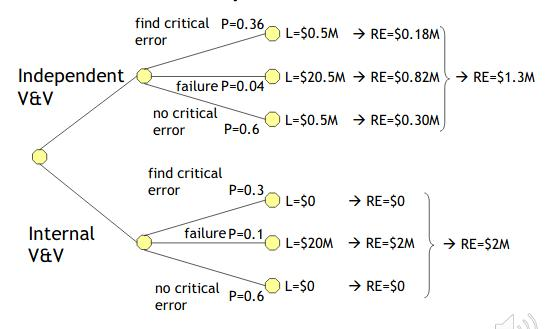
\includegraphics[scale = 0.7]{img/err.jpg}
  \caption{Esempio di decision tree}
  \label{tree}
\end{figure}
Si può fare un'\textbf{analisi di sensitività} cambiando le percentuali o i
costi al fine di ottenere un certo risultato, in modo da capire come si dovrebbe
comportare. \\
Ragionando sulle cause dei rischi usiamo il cosiddetto \textbf{risk
  tree} (esempio in figura \ref{treee}). Questo albero ha come radice il
rischio. Ogni nodo, detto 
\textbf{failure node}, è un evento che si può scomporre ``via via'' in altri
eventi, fino alle foglie. La scomposizione è guidata da due tipi di \textbf{nodi
  link}: 
\begin{enumerate}
  \item \textbf{and-node}, dove i figli di tali nodi sono eventi legati dal un
  \textit{and}
  \item \textbf{or-node}, dove i figli di tali nodi sono eventi legati dal un
  \textit{or}
\end{enumerate}
\textit{Nodi And/Or} vengono rappresentati tramite i simboli delle porte
logiche.\\
\begin{figure}
  \centering
  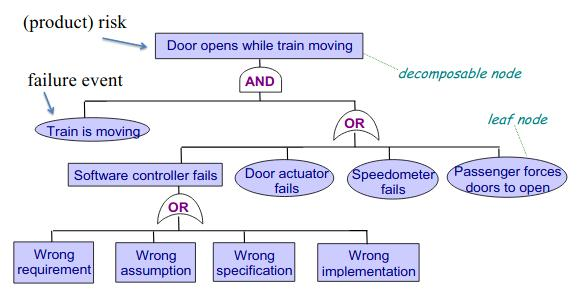
\includegraphics[scale = 0.6]{img/errr.jpg}
  \caption{Esempio di risk tree}
  \label{treee}
\end{figure}
Dato un \textit{risk tree} cerco le combinazioni di eventi atomici che possono
portare al rischio. Per farlo si esegue la \textbf{cut-set tree derivation},
ovvero, partendo dalla radice, si riporta in ogni nodo la combinazione di eventi
che possono produrre il fallimento e si vanno a calcolare le varie combinazioni
degli eventi foglia. Praticamente si deriva un insieme di eventi non
scomponibili sulle combinazioni dell'\textit{and}.
\section{Risk prioritization}
Bisogna capire quali rischi sono più ``rischiosi'' degli altri. Per farlo si
pongono i valori di $P(UO)$ e $L(UO)$ in un range, per esempio, da 1 a 10,
ricalcolando il \textit{risk exposure}. Una volta fatto si lavora in
base al \textit{risk-exposure} (che può anche essere un intervallo se le
probabilità o i costi sono in un certo intervallo). Si procede plottando i dati
su un piano con $P(UO)$ sull'asse delle $y$ e $L(UO)$ su quello delle
$x$ e facendo lo \textit{scatterplot} degli eventi (ponendoli quindi come punti
in base a $P(UO)$ e $L(UO)$). Qualora i valori siano in un range si
rappresentano con un segmento tra i due valori limite di \textit{risk
  exposure}. Con delle curve posso identificare zone di rischio diverse in base
al \textit{risk exposure} per poter catalogare gli eventi. Solitamente alla fase
di \textit{risk control} passano una decina di eventi.
\section{Risk control}
Bisogna quindi capire come gestire i rischi.\\
Per ogni rischio bisogna definire e documentare un piano specifico indicante:
\begin{itemize}
  \item cosa si sta gestendo
  \item come mitigare il rischio e quando farlo
  \item di chi è la responsabilità
  \item come approcciarsi al rischio
  \item il costo dell'approccio al rischio
\end{itemize}
Anche in questo caso ci vengono incontro liste e \textit{check-list} con le
tecniche di \textit{risk management} più comuni in base al rischio specifico.\\
Ci sono comunque strategie generali:
\begin{itemize}
  \item lavorare sulla probabilità che il rischio avvenga, sulla probabilità dei
  triggers. Bisogna capire come diminuire la probabilità
  \item lavorare, nel limite del possibile, sull'eliminazione stessa del
  rischio
  \item lavorare sulla riduzione della probabilità di avere conseguenze al
  danno, non viene quindi ridotto il rischio
  \item lavorare, nel limite del possibile, sull'eliminazione stessa del danno
  conseguente al rischio
  \item lavorare sul mitigare le conseguenze di un rischio, diminuendo l'entità
  del danno
\end{itemize}
Bisogna anche studiare le contromisure, da scegliere e attivare in base alla
situazione. Si hanno due metodi quantitativi principali per ragionare
quantitativamente sulle contromisure:
\begin{enumerate}
  \item \textbf{risk-reduction leverage}, dove si calcola quanto una certa
  contromisura può ridurre un certo rischio, secondo la seguente formula:
  \[RRL(r, cm)=\frac{RE(r)-RE\left(\frac{r}{cm}\right)}{cost(cm)}\]
      dove $r$ rappresenta il rischio, $cm$ la contromisura e $\frac{r}{cm}$ la
      contromisura $cm$ applicata al rischio $r$. Calcolo quindi la differenza
      di \textit{risk exposure} avendo e non avendo la contromisura e la divido
      per il costo della contromisura.\\
      La miglior contromisura è quella con il RRL maggiore, avendo minor costo e
      maggior efficacia dal punto di vista del \textit{risk exposure}
  \item \textbf{defect detection prevention}, più elaborato del primo è stato
  sviluppato dalla NASA. Questo metodo confronta le varie contromisure,
  confrontando anche gli obiettivi del progetto, in modo quantitativo facendo un
  confronto indiretto, producendo matrici in cui si ragiona in modo indipendente
  sulle singole contromisure e sui singoli rischi ma confrontando anche in modo
  multiplo.
  \newpage
  Si ha un ciclo a tre step:
  \begin{enumerate}
    \item elaborare la matrice di impatto dei rischi, detta \textbf{risk impact
      matrix}. Questa matrice calcola l'impatto dei rischi sugli obiettivi del
    progetto. I valori della matrice, ovvero $impact(r, obj)$ (che ha per
    colonne i rischi $r$ e righe gli obiettivi del progetto $obj$) variano da 0,
    nessun impatto, a 1, completa perdita 
    di soddisfazione (e totale non raggiungimento dell'obiettivo indicato). Ogni
    rischio viene accompagnato dalla probabilità $P$ che 
    accada. Ogni obiettivo è accompagnato dal \textbf{peso} $W$ che ha nel
    progetto (la somma di tutti i pesi è pari a 1). Si possono calcolare altri
    valori di sintesi. In primis la \textbf{criticità} di un rischio rispetto a
    tutti gli obiettivi indicati:
    \[criticality(r)=P(r)\cdot\sum_{obj}(impact(r, obj)\cdot W(obj))\]
    La criticità sale se sale l'impatto e se sale la probabilità del rischio.\\
    Un altro dato è la \textbf{perdita di raggiungimento} di un obiettivo
    qualora tutti i rischi si verificassero:
    \[loss(obj)=W(obj)\cdot\sum_{r}(impact(r, obj)\cdot P(r))\]
    
    \item elaborare contromisure efficaci per la matrice. In questa fase si usa
    il fattore di criticità del rischio. Viene prodotta una nuova matrice con
    colonne pari ai rischi (con probabilità e criticità) e righe pari alle
    contromisure. I valori saranno le riduzioni di rischio di una contromisura
    $cm$ sul rischio $r$ ($reduction(cm,r)$). La riduzione va da 0, nessuna
    riduzione, a 1, rischio eliminato. Si possono calcolare altri
    valori di sintesi. Possiamo calcolare la \textbf{combineReduction}, che ci
    dice quanto un rischio viene ridotto se tutte le contromisure sono attivate:
    \[(combineReduction(r)=1-\prod_{cm}(1-reduction(cm, r))\]
    Un altro valore è l'\textbf{overallEffect}, ovvero l'effetto di ogni
    contromisura sull'insieme dei rischi considerato:
    \[overalleffect(cm)=\sum_r(reduction(cm,r)\cdot criticality(r))\]
    si avrà effetto maggior riducendo rischi molto critici
    \item determinare il bilanciamento migliore tra riduzione dei rischi e costo
    delle contromisure. Bisogna considerare anche il costo di ogni contromisure
    e quindi si fa il rapporto tra effetto di ciascuna contromisura e il suo
    costo e scegliendo il migliore
  \end{enumerate}
\end{enumerate}
Analizzando il \textit{contingency plan} viene attuato qualora il rischio si
traduca in realtà.\\
I passa quindi al \textbf{risk monitoring/resolution}. Queste due parti sono tra
loro integrate. I rischi vanno monitorati e occorrenza vanno risolti il prima
possibile. Tutte queste attività sono costose e si lavora su un insieme limitato
di rischi, una decina.
\chapter{Capability Maturity Model Integration}
Il \textbf{Capability Maturity Model Integration (\textit{CMMI})} che è un
``programma'' di formazione e valutazione per il miglioramento a livello di
processo gestito dal \textit{CMMI Institute}.\\
Bisogna prima introdurre il concetto di \textbf{maturità dei processi}. Questa
nozione è abbastanza intuitiva. La probabilità di portare a termine un progetto
dipende dalla \textit{maturità del progetto} e la maturità dipende dal grado di
controllo che si ha sulle azioni che si vanno a svolgere per realizzare il
progetto. Si ha quindi che:
\begin{itemize}
  \item il progetto è \textbf{immaturo} quando le azioni legate allo sviluppo
  non sono ben definite o ben controllate e quindi i dev hanno troppa libertà
  che rischia di degenerare in una sorta di anarchia nel controllo del processo
  di sviluppo, alzando la probabilità di fallimento
  \item il progetto è \textbf{maturo} quando le attività svolte sono ben
  definite, chiare a tutti i partecipanti e ben controllate. Si ha quindi un
  modo per osservare quanto si sta svolgendo e verificare che sia come
  pianificato, alzando le probabilità di successo e riducendo quelle di
  fallimento
\end{itemize}
Risulta quindi essenziale ragionare sulla \textit{maturità del processo}.\\
La \textbf{maturità del processo} è definita tramite un insiemi di livelli di
maturità con associate metriche per gestire i processi, questo è detto
\textbf{Capability Maturity Model (\textit{CMM})}. In altri termini il modello
CMM è una collezione dettagliata di \textit{best practices} che aiutano le
organizzazioni a migliorare e governare tutti gli aspetti relativi al processo
di sviluppo, dalla gestione dei rischi al testing, dal design al project
management etc$\ldots$. 
\begin{center}
  \textit{Un processo migliore porta ad un prodotto migliore.}
\end{center}
La storia dei CMMs parte dagli anni novanta e porta alle versione di CMMI del
2018 che andremo ad analizzare.\\
Analizziamo quindi nel dettaglio il modello: 
\begin{figure}[H]
  \centering
  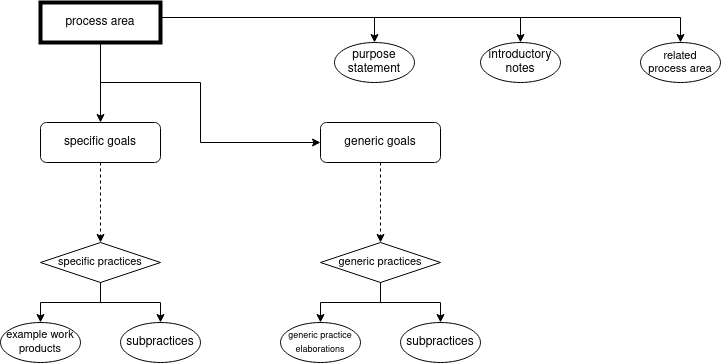
\includegraphics[scale = 0.54]{img/cmmi.png}
  \caption{Diagramma dei componenti del CMMI, secondo l'organizzazione
    standard. Nei rettangoli (tranne \textit{process area}) abbiamo i
    \textit{required}, nei rombi gli \textit{expected} e negli ovali gli
    \textit{informative}} 
  \label{fig:cmmi}
\end{figure}
All'interno del diagramma (che rappresenta letteralmente un documento) notiamo:
\begin{itemize}
  \item \textbf{process area}, che racchiude al suo interno una collezione di
  pratiche organizzate secondo obiettivi e riguarda una certa area del
  processo. Nel CMMI abbiamo 22 diverse \textit{process area}, tra cui
  \textit{configuration management}, \textit{project planning}, \textit{risk
    management} etc$\ldots$ Nel diagramma si ha lo studio di una generica
  \textit{process area}
  \item ciascuna \textbf{process area} ha:
  \begin{itemize}
    \item un \textbf{purpose statement}, che descrive lo scopo finale della
    \textit{process area} stessa
    \item un \textbf{introductory notes}, con nel note introduttive che
    descrivano i principali concetti della \textit{process area}
    \item un \textbf{related process area}, se utile, con la lista delle altre
    \textit{process area} correlate a quella corrente
  \end{itemize}
  \item le \textbf{process area} si dividono in due \textit{tipologie di
    obiettivi}:
  \begin{enumerate}
    \item \textbf{specific goals}, ovvero gli obiettivi specifici della singola
    \textit{process area} in questione. Questi obiettivi caratterizzano la
    \textit{process area}
    \item \textbf{generic goals}, ovvero gli obiettivi comuni a \textbf{tutte}
    le \textbf{process area}. Questi obiettivi rappresentano quanto la
    \textit{process area} sia ben integrata e definita nel contesto del processo
    ma questi criteri sono generali
  \end{enumerate}
  \item all'interno di ogni \textbf{specific goals} (per questo la freccia
  tratteggiata) abbiamo una serie di \textbf{specific practices}, ovvero quelle
  azioni che se svolte permettono di raggiungere quell'obiettivo specifico e, a
  loro volta, tali pratiche sono organizzate in:
  \begin{itemize}
    \item \textbf{example work product}, ovvero elenchi di esempi di prodotti
    che possono essere generati attraverso l'adempimento delle pratiche
    \item \textbf{subpractices}, ovvero pratiche di ``grana più fine''
  \end{itemize}
  \item all'interno di ogni \textbf{generic goals} (per questo la freccia
  tratteggiata) abbiamo una serie di \textbf{generic practices}, comuni a tutti,
  con le pratiche che devono essere svolte per gestire positivamente una
  qualsiasi \textit{process area} e, a loro volta, tali pratiche sono
  organizzate in:
  \begin{itemize}
    \item \textbf{generic practices elaborations}, ovvero ulteriori informazioni
    di dettaglio per la singola pratica
    \item \textbf{subpractices}, ovvero pratiche di ``grana più fine''
  \end{itemize}
  Tra i principali \textit{generic goals (GG)} abbiamo:
  \begin{itemize}
    \item \textit{GG1}: raggiungere i \textit{specific goals}, tramite
    l'esecuzione delle \textit{specific practices}
    \item \textit{GG2}: ``ufficializzare'' un \textit{managed process}, tramite
    training del personale, pianificazione del processo, controllo dei
    \textit{work product} etc$\ldots$
    \item \textit{GG3}:  ``ufficializzare'' un \textit{defined process}, tramite
    la definzione rigorosa del progetto e la raccolta di esperienze legate al
    processo
  \end{itemize}
\end{itemize}
Per capire quanto un processo software è organizzato secondo questo standard
bisogna ``mappare'' quali goals e quali pratiche si stanno perseguendo e
seguendo e usare CMMI non solo come ``ispirazione'' ma come vero e proprio
\textbf{standard} per definire le azioni da svolgere nonché per confrontare il
nostro operato e studiarlo qualitativamente. Lo studio qualitativo mi permette
di stabilire la \textbf{maturità} del progetti, secondo un certo livello di
\textit{compliance}, detto \textbf{CMMI level}. Tale qualità che può essere 
certificata da enti certificatori appositi (si ha anche una repository pubblica
con i livelli di \textit{compliance} di diversi progetti di organizzazioni
famose).\\
Studiamo a fondo questi livelli di maturità e la loro codifica.\\
Si hanno due linee di sviluppo/miglioramento:
\begin{enumerate}
  \item \textbf{capability levels (\textit{CL})}, che cattura e rappresenta
  quanto bene si sta gestendo una particolare \textit{process area} (quindi
  ciascuna \textit{process area} può raggiungere un diverso CL). Quindi per una
  singola \textit{process area} mi dice quanto bene sto raggiungendo i
  \textit{generic goals} (e di conseguenza anche i vari \textit{specific
    goals}, in quanto quelli generici impongono il controllo di quelli
  specifici). A livello di grafico punta all'ovale con \textit{specific goals}.
  Il CL ha valore da 0 a 3:
  \begin{itemize}
    \item \textbf{level 0: \textit{incomplete}}, dove probabilmente non si
    stanno nemmeno svolgendo tutte le pratiche richieste per quella
    \textit{process area} o sono state svolte solo parzialmente
    \item \textbf{level 1: \textit{performed}}, dove si eseguono le pratiche e i
    vari \textit{specific goals} sono soddisfatti
    \item \textbf{level 2: \textit{managed}}, dove oltre alle pratiche si ha
    anche una gestione (controllo, allocazione di risorse, monitoring, review
    etc$\ldots$) delle attività stesse, come indicato nello standard. Si ha una
    policy per l'esecuzione delle pratiche 
    \item \textbf{level 3: \textit{defined}}, dove l'intero processo è ben
    definito secondo lo standard, descritto rigorosamente e si ha un processo
    completamente su misura dell'organizzazione 
  \end{itemize}
  I CL di ciascuna \textit{process area} possono essere rappresentate su un
  diagramma a barre, dove viene indicato il CL attuale e il \textbf{profile
    target}, ovvero il livello a cui quella \textit{process area} deve
  arrivare (che non è per forza il terzo).
  \item \textbf{maturity levels (\textit{ML})}, che cattura il livello raggiunto
  dall'intero processo di sviluppo ragionando su tutte le \textit{process area}
  attivate. Rappresenta quanto bene si sta lavorando sull'insieme intero della
  \textit{process area}. A livello di grafico punta direttamente all'elemento
  specificante la \textit{process area}. Il ML ha valore da 1 a 5:
    \begin{itemize}
    \item \textbf{level 1: \textit{initial}}, dove si ha un processo gestito in
    modo caotico
    \item \textbf{level 2: \textit{managed}}, dove si ha già un processo ben
    gestito secondo varie policy
    \item \textbf{level 3: \textit{defined}}, dove si ha un processo ben
    definito secondo lo standard aziendale
    \item \textbf{level 4: \textit{quantitatively managed}}, dove si stanno
    anche raccogliendo dati che misurano quanto bene sta funzionando il
    processo, facendo quindi una misura quantitativa dello stesso
    \item \textbf{level 5: \textit{optimizing}}, dove grazie alle informazioni
    raccolte nel livello precedente ottimizzo il processo, in un'idea di
    \textit{continuous improvement} del progetto stesso
  \end{itemize}
  Gli ultimi due livelli sono davvero difficili da raggiungere.
\end{enumerate}
Rapportiamo quindi CL e ML in base  avari blocchi di \textit{process area}, che
scalano per ``importanza'':
\begin{itemize}
  \item il processo è a ML=2 se tutte le \textit{process area} del blocco (che
  si riferisce alle \textit{process area} riferite al blocco \textit{planned \&
    executed}) sono svolte tutte a CL=2
  \item il processo è a ML=3 se aggiungo le \textit{process area} del blocco
  \textit{org. standard} e queste sono tutte a CL=3 
  \item il processo è a ML=4 se aggiungo le due \textit{process area} del blocco
  \textit{quantitative PM} che devono essere svolte a CL=3
  \item il processo è a ML=5 se aggiungo le ultime due \textit{process area},
  ovvero quelle del blocco \textit{continuous improvement}, che devono essere
  svolte a CL=3 
\end{itemize}
Si possono confrontare CMMI e le pratiche agili.\\
Ciò che viene svolto ai livelli 2 e 3 (con qualche piccolo adattamento) di
\textit{maturity level} si fa ciò che viene fatto anche coi metodi agili. In
merito ai livelli 4 e 5 di \textit{maturity level} si hanno pratiche che non
rientrano nell'ottica dei metodi agili. Quindi un'organizzazione può usare i
metodi agili ed essere standardizzata rispetto CMMI raggiungendo un
\textit{maturity level} 2 o 3.\\
CMMI è quindi uno standard industriale con certificazioni ufficiali.
\chapter{Requirements engineering}
Quando si parla di \textbf{requirements engineering (\textit{RE},
  ingegnerizzazione dei requisiti)} di fatto ci si concentra sulla comprensione
di come una soluzione software si deve comportare per risolvere un certo
problema. In questo senso bisogna prima comprendere quale sia il\textbf{
  problema} da risolvere e in quale \textbf{contesto} tale problema si verifica,
per poter arrivare ad una soluzione corretta ed efficacie a problemi
``reali''. Bisogna ben comprendere il problema, non si parla quindi della
progettazione in se, ma del ``cosa'' deve fare il software.
\begin{esempio}
  Vediamo un esempio banale.\\
  Bisogna sviluppare il software per l'\textit{adaptive cruise control}. In
  questo caso si ha:
  \begin{itemize}
    \item il \textit{problema} che consiste nel seguire correttamente la
    macchina che si ha davanti in autostrada
    \item il \textit{contesto} che consiste in:
    \begin{itemize}
      \item guida della macchina
      \item intenzioni del guidatore
      \item norme di sicurezza
      \item etc$\ldots$
    \end{itemize}
  \end{itemize}
\end{esempio}
\begin{esempio}
  Vediamo ora l'analogia classica per spiegare il RE, il \textup{problema mondo}
  e la \textup{soluzione macchina}.\\
  Si hanno:
  \begin{itemize}
    \item il \textbf{mondo}, con un problema derivante dal mondo reale, mondo
    stesso che produce tale problema che bisognerà risolvere con un
    calcolatore. Si hanno all'interno:
    \begin{itemize}
      \item \textup{componenti umane}, ovvero staff, operatori, organizzazioni
      etc$\ldots$
      \item \textup{componenti fisiche}, ovvero device, software legacy, madre
      natura etc$\ldots$
    \end{itemize}
    \item la \textbf{macchina}, che bisogna sviluppare per risolvere il
    problema. Si ha necessità quindi di:
    \begin{itemize}
      \item \textup{software} da sviluppare o acquistare
      \item \textup{piattaforma hardware/software}, con eventuali device annessi
    \end{itemize}
    
    \item \textup{requirements engineering} che si occupa di:
    \begin{itemize}
      \item definire gli effetti della \textup{macchina} sul problema del
      \textup{mondo} 
      \item definire assunzioni e proprietà principali del \textup{mondo} stesso
    \end{itemize}
  \end{itemize}
  Macchina e mondo possono condividere alcuni componenti, con la macchina che
  modifica il mondo (nell'esempio precedente la macchina che disattiva il cruise
  control agisce sia a livello software che a livello del mondo esterno). Nei RE
  studiamo quindi il \textup{mondo}, senza definire come funziona internamente
  la macchina (nelle parti che non interagiscono direttamente col mondo, per
  esempio scelte di design etc\ldots).
\end{esempio}
Quando si parla di RE è bene distinguere due elementi:
\begin{enumerate}
  \item ogni volta che prendiamo in consideriamo un problema esiste sempre un
  \textbf{system-as-is}, ovvero un sistema preesistente che già risolve il
  problema (anche se magari in modo non efficiente o qualitativamente
  sufficiente). Si ha quindi sempre un sistema da cui partire (esempio banale
  per il cruise control è dire che in realtà la soluzione al problema già esiste
  con la guida senza cruise control)
  \item esiste sempre un \textbf{system-to-be}, ovvero il sistema che si andrà a
  realizzare. In altre parole è il sistema quando la \textit{macchina/software}
  ci opera sopra
\end{enumerate}
Studiare il \textit{system-as-is} è essenziale per poter lavorare al
\textit{system-to-be}.
\newpage
\begin{definizione}
  Il requirements engineering è, formalmente, un insieme di attività:
  \begin{itemize}
    \item per esplorare, valutare, documentare, consolidare, rivisitare e
    adattare gli obiettivi, le capacità, le qualità, i vincoli e le ipotesi su
    un \textup{system-to-be} 
    \item basate sul problema sorto dal \textit{system-as-is} e sulle nuove
    opportunità tecnologiche
  \end{itemize}
  L'output di queste attività è un \textbf{documento di specifica dei requisiti}
  con tutto ciò che soddisfa il sistema. Se l'output non è un singolo documento
  si ha una collezione di singoli requisiti, che nel metodo agile sono
  \textit{storie/cards} e in altri metodi un repository centrale con un db
  condiviso contenete i vari requisiti.\\
  In ogni caso si ha un insieme di requisiti su come si deve comportare il
  sistema che si realizza, descrivendo quanto descritto nei punti precedenti.
\end{definizione}
In un modello simil-cascata di sviluppo software il RE è una delle primissime
attività, subito dopo quelle di definizione del sistema e di business plan. Per
gli aspetti tecnici è probabilmente la prima attività svolta, occupandosi di
\textit{ottenere il giusto sistema da sviluppare (per fare la cosa giusto)},
prima di design, 
implementazione ed evoluzione software etc$\ldots$ che si occupano di
\textit{ottenere il software giusto, sviluppandolo nel modo corretto}.\\
Errare nel RE può portare ad un ottimo software che risolve i problemi sbagliati
(o non tutti i problemi che dovrebbe risolvere). Sbagliare i RE è una causa di
fallimento del progetto (anche in un contesto non agile).\\
Lavorare sui RE non è semplice per diversi motivi:
\begin{itemize}
  \item si deve ragionare su tante versioni del sistema:
  \begin{itemize}
    \item as-is
    \item to-be
    \item to-be-next, volendo essere lungimiranti per il comportamento del
    sistema, sapendo e prevedendo evoluzioni future
  \end{itemize}
  \item si lavora in \textit{ambienti ibridi}, tra umani, leggi, device, policy,
  leggi della fisica, etc$\ldots$, quindi in un contesto eterogeneo che va
  compreso a fondo (ignorare degli aspetti può portare al fallimento)
  \item si hanno diversi aspetti funzionali, qualitativi e di sviluppo
  \item si hanno diversi livelli di astrazione, con obiettivi strategici a lungo
  termine di inserimento sul mercato e dettagli operazionali
  \item si hanno tanti stakeholders, quindi con diverse parti interessati di cui
  risolvere problemi e interessi (con potenziali conflitti tra i vari
  stakeholders)
  \item si hanno tante attività tecniche legate l'una con l'altra:
  \begin{itemize}
    \item conflict management
    \item risk management
    \item evaluation of alternatives
    \item prioritization
    \item quality assurance
    \item change anticipation
  \end{itemize}
  per capire cosa fare, in che ordine, con che rischi, che livelli di qualità,
  etc$\ldots$
\end{itemize}
\section{Tipi di requisiti}
Bisogna anche ragioni sui tipi di requisiti su cui si deve lavorare.\\
Una prima differenza si ha nel modo in cui sono scritti i requisiti. Si hanno
quindi:
\begin{itemize}
  \item \textbf{descriptive statements (\textit{dichiarazioni descrittive})},
  che indicano dei requisiti non negoziabili, rappresentano dei comportamenti
  derivanti dalle leggi del mondo su cui lavora la macchina. Si ha quindi zero
  margine di modifica
  \item \textbf{prescriptive statements (\textit{dichiarazioni prescrittive})},
  che indicano requisiti negoziabili
\end{itemize}
\begin{esempio}
  Vediamo un esempio.\\
  Per il primo modo si ha:
  \begin{center}
    \textit{La stessa copia non può essere presa in prestito da due persone
      diverse contemporaneamente}
  \end{center}
  per il secondo:
  \begin{center}
    \textit{Un cliente abituale non può prendere in prestito più di tre libri
      contemporaneamente}
  \end{center}
\end{esempio}
Entrambi sono importanti e vanno considerati. Si possono avere requisiti non
ovvi, o lo sono in un contesto specialistico e quindi spesso non ovvi a chi
lavora sul software (che generalmente non è del settore specialistico), che
magari nemmeno sa che esistono.\\
I requisiti possono inoltre differire per gli elementi che prendono in
considerazione. Posso avere requisti:
\begin{itemize}
  \item \textbf{system requirements}, che riguardano come si comporta
  l'ambiente, per capirne il funzionamento (che andrà ad influenzare il
  software) 
  \item \textbf{software requirements} che studiano come si comporta il software
  nell'ambiente, studiando i cosiddetti \textit{shared fenomena}
\end{itemize}
ricordando che:
\[sistema = ambiente + software\]
\textit{I requisti comunque non riguardano mai il comportamento interno del
  software (variabili, error code etc$\ldots$)}.\\
Si hanno 3 dimensioni:
\begin{enumerate}
  \item \textbf{dimensione del why}, dove si identificano, analizzano e
  rifiniscono i requisiti del \textbf{system-to-be} per:
  affrontare le carenze analizzate del \textbf{system-as-is}, in linea con gli
  obiettivi di business, sfruttando le opportunità tecnologiche.\\
  Si hanno le seguenti difficoltà:
  \begin{itemize}
    \item acquisire conoscenza del dominio 
    \item valutare opzioni alternative (ad esempio modi alternativi per
    soddisfare lo stesso obiettivo) 
    \item abbinare problemi-opportunità e valutarli in termini di implicazioni,
    e rischi associati 
    \item gestire obiettivi contrastanti
  \end{itemize}

  \item \textbf{dimensione del what}, dove si identificano, analizzano e
  rifiniscono le funzionalità del \textbf{system-to-be} (servizi software e
  associate procedure manuali) per soddisfare gli obiettivi individuati in
  base a vincoli di qualità: sicurezza, prestazioni, etc$\ldots $basati su
  ipotesi realistiche sull'ambiente.\\
  Si hanno le seguenti difficoltà:
  \begin{itemize}
    \item identificare il giusto set di funzionalità 
    \item specificarle precisamente per essere comprese da tutte le parti 
    \item garantire la tracciabilità $backward$ per gli obiettivi del sistema
  \end{itemize}
  \item \textbf{dimensione del who}, dove si assegnaresponsabilità per gli
  obiettivi, i servizi, i vincoli tra i componenti del \textbf{system-to-be} in
  base alle loro capacità e agli obiettivi del sistema, oltre i confini
  dell'ambiente software.\\
  La difficoltà è valutare opzioni alternative per decidere il giusto grado di
  automazione 
\end{enumerate}
I requisti che riguardano l'ambiente possono essere di due forme:
\begin{enumerate}
  \item \textbf{domain properties}, ovvero proprietà riguardanti l'ambiente,
  immutabili
  \item \textbf{assumptions}, ovvero le assunzioni fatte su come è fatto
  l'ambiente. Il software funzionerà solo negli ambienti che soddisfano quella
  certa assunzione (per esempio un numero massimo di chiamate API a cui il
  sistema è in grado di rispondere). Le assunzioni descrivono gli ambienti
  compatibili con il software. Se troppo restrittive possono portare al
  fallimento del progetto, che riguarderebbe pochissimi casi particolari
\end{enumerate}
In ottica di un ragionamento di interazione tra sistema software e ambiente
citiamo il \textbf{modello Parnas95}, della metà degli anni novanta. 
\begin{figure}
  \centering
  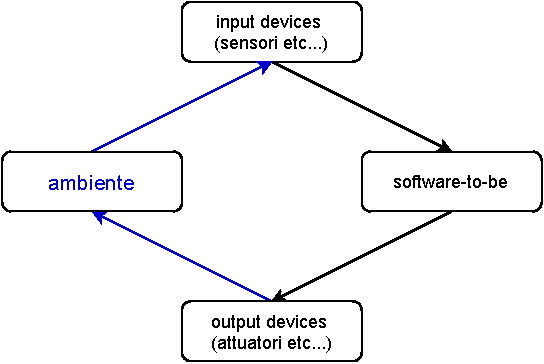
\includegraphics[scale = 0.7]{img/re.pdf}
  \caption{Raffigurazione del modello Parnas95}
\end{figure}
\newpage
In modo elementare il modello schematizza
questa interazione software-ambiente in modo da esplicitare i device usati dal
software-to-be per interagire con ambiente. Si ha uno schema composto da 4
elementi:

\begin{enumerate}
  \item dei device di input, simil sensori, che percepiscono l'ambiente (ad
  esempio richieste che arrivano dal web)
  \item dei device di output che permettono di interagire con l'ambiente (che
  possono ad esempio essere le risposte renderizzate nel browser)
\end{enumerate}
Si hanno 4 tipi di variabili:
\begin{enumerate}
  \item \textbf{input data (I)}, tra \textit{input devices} e
  \textit{software-to-be}
  \item \textbf{output results (O)}, tra \textit{software-to-be} e
  \textit{output devices}
  \item \textbf{controlled variables  (C)}, tra \textit{output devices} e
  \textit{ambiente}
  \item \textbf{monitored variables (M)}, tra \textit{ambiente} e
  \textit{input devices}
\end{enumerate}
Si ha che:
\[\mbox{System requirements}\subseteq M\times C\]
\[\mbox{Software requirements}\subseteq I\times O\]

\[\mbox{Assumptions}\subseteq M\times C\cup M\times i\cup C\times O\]
Nel caso, ad esempio, di sistemi embedded, di domotica o simili tali device
diventano parecchio complessi.\\
\begin{definizione}
  Definiamo \textbf{domain property} come un \textit{descriptive statement} sui
  problemi legati ai fenomeni del \textit{mondo} (a prescindere da qualsiasi
  \textbf{software-to-be}).\\
  \[\mbox{Domain property}\subseteq M\times C \mbox{ se leggi che non possono
      essere infrante}\]
\end{definizione}
Si ha che:
\[\mbox{Software requirements}= \]
\[\footnotesize{map}(\mbox{\footnotesize{System requirements, Software
      requirements,  Domain property}})\]
\textbf{esempi su slide}.\\

È utile quindi fare una distinzione per quanto concerne i requisiti del
software. Abbiamo due famiglie principali:
\begin{enumerate}
  \item \textbf{requisiti funzionali}, che indicano le funzionalità che un
  sistema, \textit{system-to-be}, deve implementare, cosa deve essere in grado
  di fare. Non sono prevedibili prima di studiare il sistema
  \item \textbf{requisiti non funzionali}, che indicano delle qualità o dei
  vincoli sulle funzionalità e quindi sui requisiti funzionali. Possono essere
  in termini di prestazioni, sicurezza, qualità etc$\ldots$ delle
  funzionalità. Questa famiglia di aspetti non funzionali è più o meno standard
\end{enumerate}
\begin{esempio}
  Posso avere il requisito funzionale:
  \begin{center}
    \textit{Il cliente è in grado di prendere in prestito al massimo tre libri}
  \end{center}
  e quello non funzionale:
  \begin{center}
    \textit{Un cliente può prendere in prestito i libri solo dopo il
      riconoscimento}  
  \end{center}
\end{esempio}
Si ha quindi una tassonomia dove si trovano organizzati aspetti non funzionali
tali per cui, dopo aver individuato le funzionalità, possono essere usate per
chiedersi se, per ciascun aspetto, esso è rilevante, individuando nuovi requisiti
non funzionali da includere nell'insieme dei requisiti.\\
Per alcuni tipi di progetti requisiti funzionali e non sono difficilmente
distinguibili, spesso mischiandosi (si pensi, ad esempio, alla sicurezza nello
sviluppo dio un firewall).
\begin{figure}[H]
  \centering
  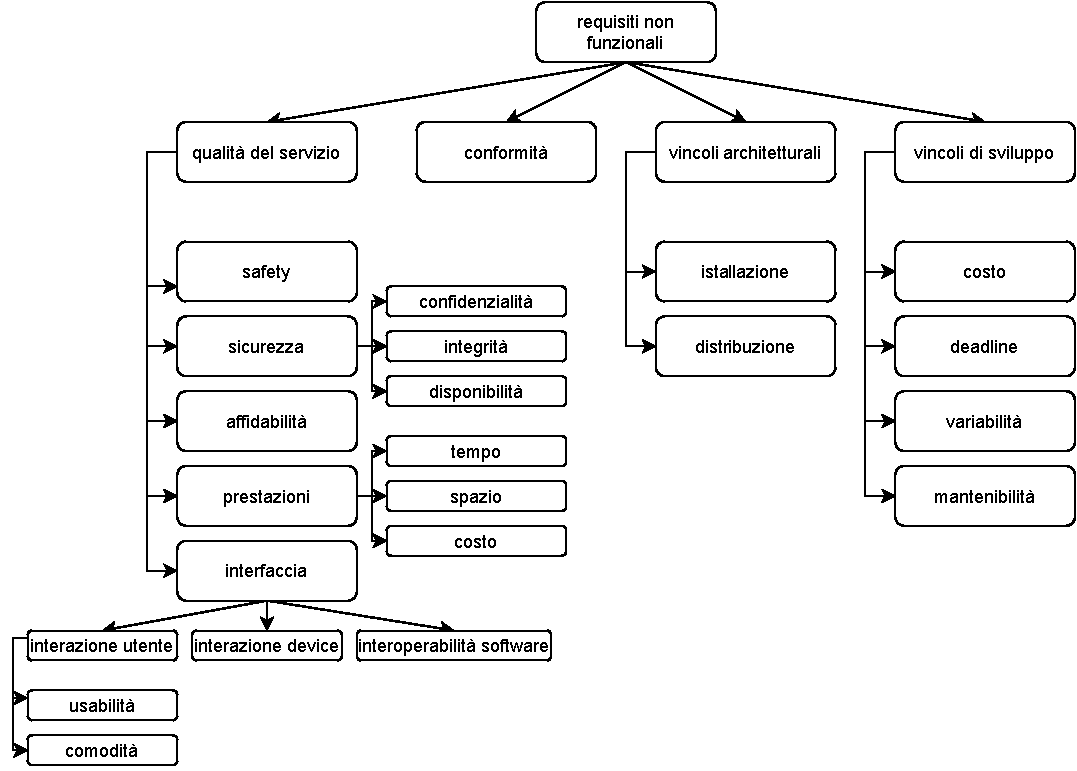
\includegraphics[scale = 0.7]{img/re2.pdf}
  \caption{Tassonomia dei requisiti non funzionali}
\end{figure}

\section{Qualità dei requisiti}
Si hanno diversi aspetti di cui preoccuparsi nell'analisi dei requisiti. Si
hanno tante qualità indispensabili:
\begin{itemize}
  \item \textbf{completezza} di quanto descriviamo, descrivendo tutti i
  requisiti rilevanti del progetto, identificando tutti i comportamenti del
  sistema e documentarli in modo adeguato. È una qualità virtualmente
  irraggiungibile in modo assoluto, non è infatti verificabile. Inoltre i
  requisiti variano al proseguire del progetto, interagendo anche con gli
  stakeholders, rendendo questo uno degli aspetti più difficili da studiare
  \item \textbf{consistenza} dei requisti, senza conflitti. Nella mole di
  requisiti si possono purtroppo facilmente introdurre inconsistenze
  \item \textbf{non ambiguità} di ciò che si scrive. Tutto deve essere chiaro e
  non soggetto ad interpretazione
  \item \textbf{misurabilità}, quando rilevante, e quindi non basato su
  interpretazioni vaghe ma si misure concrete e specifiche 
  \item \textbf{fattibilità}, ovvero non si devono avere requisiti basati su
  funzionalità irrealizzabili
  \item \textbf{comprensibilità}
  \item \textbf{buona struttura}
  \item \textbf{modificabilità}, con possibilità di avere il risultato
  mantenibile del tempo 
  \item \textbf{tracciabilità}, individuando tutti gli artefatti ottenibili come
  conseguenza e tracciandoli. Si tracciano anche le dipendenze tra requisiti
\end{itemize}
Vediamo quindi gli errori che si fanno quando si va ad identificare i requisiti,
per poter poi studiare tecniche per evitare, nel limite del possibile, tali
errori:
\begin{itemize}
  \item \textbf{omissioni}, non riuscendo ad identificare qualche
  requisito. Anche un riconoscimento tardivo è un problema in quanto comporta la
  modifica del documento, non sempre facile
  \item \textbf{contraddizioni}, avendo conflitti tra i requisiti (anche solo,
  banalmente, per i requisiti di un treno si potrebbe avere che non si possono
  aprire le porte tra due stazioni ma anche se si possono aprire le porte in
  caso d'emergenza) 
  \item \textbf{inadeguatezza}, avendo requisiti che non sono adeguati per
  un determinato problema
  \item \textbf{ambiguità}, avendo requisiti interpretabili
  \item \textbf{non misurabilità} di certi requisiti (specialmente non
  funzionali), che comportano difficoltà di gestione, precludendo confronti
  etc$\ldots$ 
\end{itemize}
Si hanno anche altri tipi di errore:
\begin{itemize}
  \item essere \textbf{troppo specifici} nella definizione dei requisiti
  includendo anche comportamenti interni al software che non dovrebbero essere
  descritti in questa fase. Bisogna dire quali funzionalità bisogna realizzare,
  non come
  \item descrivere requisiti \textbf{non implementabili} considerando vincoli
  temporali o di costo
  \item descrivere requisti \textbf{complessi da leggere}, ad esempio con un uso
  eccessivo di acronimi
  \item avere \textbf{poca struttura} nella stesura dei requisiti, a livello
  visivo. Un documento tecnico deve essere facile da gestire e da usare
  \item se si produce un documento (e non nel caso dell'uso del db) bisogna
  evitare di fare riferimento a requisiti che non sono stati ancora descritti,
  ovvero evitando il \textbf{forward reference}
  \item evitare ``\textbf{rimorsi}'' di non aver definito nel momento giusto
  certi concetti che magari erano stati usati, senza definizione,
  precedentemente. Questi vanno definiti all'inizio del documento (nelle slide
  si dice tra parentesi)
  \item evitare la \textbf{poco modificabilità} del documento. È buona norma
  avere delle ``costanti simboliche'', definite all'inizio, a cui fare
  riferimento nel documento, in modo che un'eventuale modifica si rifletta su
  tutto il documento
  \item evitare l'\textbf{opacità/logica di fondo/rationale/motivazioni} dei
  requisti, in modo che sia 
  chiaro il perché esso è stato incluso, portando a mettere in discussione
  requisiti in realtà sensati a cui si arriverebbe comunque dopo ulteriore
  analisi, dopo aver perso ulteriore tempo
  
\end{itemize}
\section{Il processo RE}
Vediamo le principali fasi del RE.\\
Si hanno 4 fasi a spirale:
\begin{enumerate}
  \item \textbf{domain understanding \& elicitation}
  \item \textbf{evaluation \& agreement}
  \item \textbf{specification \& documentation}
  \item \textbf{validation \& verification}
\end{enumerate}
\begin{figure}
  \centering
  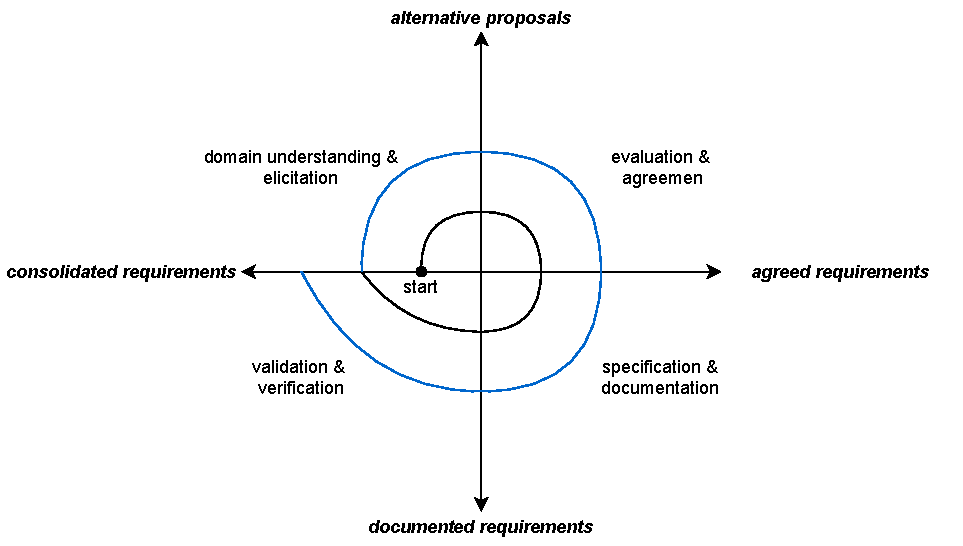
\includegraphics[scale = 0.8]{img/re3.pdf}
  \caption{Rappresentazione a spirale delle quattro fasi del RE}
\end{figure}
\paragraph{domain understanding \& elicitation}
In questa fase si hanno due parti principali:
\begin{enumerate}
  \item \textbf{domain understanding}
  \item \textbf{requirements elicitation}
\end{enumerate}
\newpage
Nella \textit{domain understanding} si ha:
\begin{itemize}
  \item lo studio del \textit{system-as-is} in ottica di studio del dominio
  applicativo, studio del business organizzazione che vuole il prodotto. Si
  studiano anche forze e debolezze del \textit{system-as-is}. Si studia il
  dominio applicativo, spesso sconosciuto e complesso, per ottenere il miglior
  \textit{system-to-be} possibile
  \item si identificano gli stakeholders (e quindi tutte le parti interessate)
  del progetto per poter capire a fondo interessi e fini
\end{itemize}
Come \textbf{output} della \textit{domain understanding} si hanno:
\begin{itemize}
  \item le sezioni iniziali per la bozza di proposta preliminare
  \item il glossario dei termini
\end{itemize}
Passando alla \textit{requirements elicitation} si uno studio più approfondito
nel mondo:
\begin{itemize}
  \item si ha un'ulteriore analisi dei problemi legati al \textit{system-as-is},
  alla ricerca di sintomi, cause e conseguenze
  \item vengono identificati, grazie all'aiuto degli stakeholders:
  \begin{itemize}
    \item opportunità tecnologiche
    \item condizioni del mercato
    \item obiettivi di miglioramento
    \item vincoli, organizzativi e tecnici, del \textit{system-as-is}
    \item alternative per raggiungere l'obiettivo e assegnare le responsabilità
    \item scenari di ipotetica interazione software-ambiente
    \item requisiti del software
    \item assunzioni sull'ambiente
  \end{itemize}
\end{itemize}
In \textbf{in output} alla \textit{requirements elicitation} si hanno ulteriori
sezioni per la bozza di proposta preliminare

\paragraph{evaluation \& agreement}
Come risultato nella fase precedente si effettuando decisioni basate
sull'interazione con i vari stakeholders (che spesso richiedono funzionalità
conflittuali etc$\ldots$), per poter valutare e decidere, avendo cambiamenti
dei rischi in base a:
\begin{itemize}
  \item identificazione e risoluzione di conflitti di interesse
  \item identificazione e risoluzione di rischi legati al sistema proposto
  \item comparazione e scelta tra le alternative proposte in merito a obiettivi
  e rischi
  \item prioritizzazione dei requisti, al fine di:
  \begin{itemize}
    \item risolvere conflitti
    \item definire vincoli di costi e tempi
    \item supportare lo sviluppo incrementale
  \end{itemize}
\end{itemize}
In \textbf{in output} a questa fase si hanno le sezioni finali per la bozza di
proposta preliminare, dove si documentano gli obiettivi selezionati, i
requisiti, le assunzioni e il \textit{rationale}, la logica di fondo delle
opzioni selezionate 
\paragraph{specification \& documentation}
In questa fase si raccoglie quanto detto nelle prime due fasi per produrre il
documento, si hanno quindi:
\begin{itemize}
  \item definizione precisa di tutte le funzionalità del sistema scelto, tra
  cui: 
  \begin{itemize}
    \item obiettivi, concetti, proprietà rilevanti del dominio d'interesse,
    requisti del sistema, requisti del software, assunzioni sull'ambiente e
    responsabilità
    \item motivazioni e logica di fondo delle opzioni scelte
    \item probabili evoluzioni del sistema ed eventuali variazioni
  \end{itemize}
  \item organizzazione di quanto appena citato in una struttura coerente
  \item documentazione del tutto in un formato comprensibile a tutte le parti,
  mettendo in allegato:
  \begin{itemize}
    \item costi
    \item piano di lavoro
    \item tempi di consegna del risultato
  \end{itemize}
\end{itemize}
In \textbf{output} a questa fase si ha il vero e proprio \textbf{Requirements
  Document (\textit{RD})}
\paragraph{validation \& verification}
In questa fase si studia l'RD, ovvero si studia la garanzia di qualità dell'RD
(in modo equivalente a quanto può essere fatto durante la produzione di un
software1, analizzando varie attività: 
\begin{itemize}
  \item \textbf{validazione}, ovvero vedendo se quanto contenuto nell'RD è
  adeguato con quanto si necessita
  \item \textbf{verifica}, controllando se ci sono omissioni o inconsistenze
  \item \textbf{correzione} di eventuali errori e difetti
\end{itemize}
In \textbf{output} a questa fase si ha un RD consolidato.
\paragraph{Ciclicità del processo}
Come è stato detto queste quattro fasi si ripetono in modo iterativo in modo ``a
spirale''. Questo viene fatto in quanto si possono avere evoluzioni nel processo
nonché correzioni di quanto già fatto che si propagano su tutto il documento. Le
evoluzioni e le correzioni possono sopraggiungere durante:
\begin{itemize}
  \item il RE stesso
  \item lo sviluppo del software
  \item dopo il deploy del software stesso
\end{itemize}
Dopo ogni ciclo si è molto più consci del sistema e si può passare al
miglioramento del RE con più efficacia.\\
Questo sistema è molto compatibile con i vari \textbf{metodi agili}.
\subsection{Domain understanding \& elicitation}
Approfondiamo questa fase analizzando i vari aspetti. Partiamo con la tecnica
dell'\textbf{elicitation}, che consiste in tecniche atte allo scoprire requisiti
che un progetto deve soddisfare. 
\subsubsection{Stakeholders}
La prima parte è la selezione degli stakeholders del progetto. Questa fase è la
prima che viene svolta per poter lavorare alla \textit{elicitation}. In generale
uno stakeholder è un'organizzazione o una persona che nutre un interesse
rispetto al progetto. Conoscendo gli stakeholders avremo modo di prendere in
considerazioni gli interessi degli stakeholders tramite diverse
strategie. Idealmente si vuole realizzare qualcosa che soddisfi tutti gli
interessi di tutti gli stakeholders.\\
I hanno diversi aspetti per la selezione degli stessi:
\begin{itemize}
  \item posizione nell'organizzazione
  \item ruolo nel prendere decisioni sul \textit{system-to-be}
  \item livello di esperienza del dominio applicativo
  \item esposizione al problema che il sistema deve risolvere
  \item influenza nell'accettazione del sistema
  \item obiettivi personali ed eventuali conflitti di interesse
\end{itemize}
Questa è un'attività insidiosa in quanto non si può dire se l'insieme degli
stakeholders sia completo.\\
Si hanno anche stakeholders non sono dell'organizzazione ma anche associazioni,
ulteriori organizzazioni,
addetti alle normative di settore etc$\ldots$ producendo un insieme molto ampio
e variegato, proporzionalmente alla grandezza del progetto. Si hanno anche
stakeholders che non interagiscono direttamente col sistema.\\
Un modo per identificare gli stakeholders è tramite una serie di semplici
domande, tramite una piccola attività di brainstorming (da fare anche insieme ad
analisti):
\begin{itemize}
  \item chi è influenzato positivamente e negativamente dal progetto? 
  \item chi ha il potere di fargli avere successo (o farlo fallire)? 
  \item chi prende le decisioni in materia di denaro? 
  \item chi sono i fornitori? 
  \item chi sono gli utenti finali? 
  \item chi ha influenza, anche indiretta, sugli altri stakeholder? 
  \item chi potrebbe risolvere potenziali problemi con il progetto? 
  \item chi si occupa di assegnare o procurare risorse o strutture? 
  \item chi ha competenze specialistiche cruciali per il progetto?
\end{itemize}
Si hanno vari check-list simili online.\\
Dimenticare uno stakeholders può portare ritardi o fallimenti del progetto,
dovendo rivedere magari requisti (specifici di quello stakeholder) o dovendo
rifare parti di sviluppo.\\ 
Si hanno varie difficoltà nell'acquisire informazioni dagli stakeholders,
rendendo complesso il dialogo:
\begin{itemize}
  \item fonti di conoscenza sul sistema distribuite sui vari stakeholders e tali
  fonti spesso sono contrastanti 
  \item accesso difficile alle fonti 
  \item ostacoli alla buona comunicazione, avendo background diversi sul dominio
  \item conoscenza non comunicata esplicitamente (magari anche solo perché date
  per scontate dagli esperti di un certo dominio o perché alcune informazioni
  sono sensibili o segretate) e bisogni nascosti
  \item fattori socio-politici 
  \item condizioni instabili e mutabili, cambiano gli stakeholders, si hanno
  dinamiche aziendale mutevoli e cambi di ruoli. Anche per questo si hanno i
  metodi agili
\end{itemize}
Serve molta esperienza per gestire queste situazioni.\\
Servono quindi \textbf{buone capacità comunicative}, sapendo usare la giusta
terminologia di dominio (ovvero quella dello stakeholders), arrivando dritti al
punto e creando un rapporto di fiducia con gli stakeholders.\\
Si ha inoltre un piccola pratica, detta \textit{knowledge reformulation}, ovvero
quando si acquisiscono informazioni anche da fonti multiple è bene riformulare
tale informazione allo stakeholder, per verificare una corretta comprensione.\\
È bene fare distinzione sulle tecniche di engagement con gli stakeholders,
considerando due variabili, catalogandole in $low$ e $high$:
\begin{enumerate}
  \item potere decisionale
  \item interesse nel progetto
\end{enumerate}
Si ha quindi:
\begin{table}[H]
  \centering
  \begin{tabular}{c|c|c}
    potere & interesse & strategia\\
    \hline
    high & high & fully engage\\
    high & low & keep satisfied\\
    low & high & keep satisfied\\
    low & low & minimum effort
  \end{tabular}
\end{table}
Dove nel dettaglio:
\begin{itemize}
  \item \textbf{fully engage}: ovvero coinvolgimento regolare degli stakeholders
  che in questo caso sono della categoria principale. Devono essere
  estremamente soddisfatti
  \item \textbf{keep satisfied}: si hanno due casi:
  \begin{itemize}
    \item se hanno alto potere decisionale si cerca di mantenerli informati e
    soddisfatti ma senza troppi dettagli
    \item se hanno alto interesse, essendo spesso gli end-user, si cerca di
    consultarli spesso cercando di risolvere le problematiche indicate,
    coinvolgendoli regolarmente per ottenere dettagli e informazioni specifiche,
    essendo spesso i più informati sui dettagli
  \end{itemize}
  \item \textbf{minimum effort}: mentendoli informati in modo generale e
  monitorandone eventuali cambi di ruolo, potere o interesse
\end{itemize}
\subsubsection{Elicitation techniques}
Passiamo quindi alle tecniche di elicitation. Si hanno due famiglie principali:
\begin{itemize}
  \item \textbf{artefact-driven}, che fanno uso di artefatti per poter scoprire
  requisiti
  \item \textbf{stakeholders-driven}, che fanno invece uso degli stakeholders
\end{itemize}
\paragraph{Artefact-driven}
La prima tecnica è il \textbf{background study}, ovvero collezionare leggere e
sintetizzare documenti su:
\begin{itemize}
  \item le \textbf{organizzazioni stesse}, ovvero grafici, business plan, report
  finanziari, tempi delle riunioni etc$\ldots$
  \item il \textbf{dominio applicativo}, ovvero libri, paper, report su sistemi
  simili etc$\ldots$
  \item il \textbf{system-as-is}, ovvero workflow documentati, procedure, regole
  di business, report di errori, richieste di cambiamenti etc$\ldots$
\end{itemize}
Queste collezioni di dati ci permettono di informarci in modo autonomo sul mondo
in cui si andrà a lavorare, senza coinvolgere lo stakeholders, in quanto
costoso, dispendioso e limitato in termini di tempo. Gli stakeholders vanno
interpellati non per informazioni reperibili autonomamente ma per estrarre
conoscenza non pubblica e non documentata. Ci si presenta allo stakeholder già
con una base di conoscenza e conoscendo già la terminologia corretta del
dominio. \\
Si ha quindi l'attività di \textbf{data collection} dove si estraggono
informazioni dai dati di marketing, statistici etc$\ldots$ Sono dati utili per
studiare il target. Si possono fare attività di \textit{survey}. Si collezionano
dati anche già documentati.\\
L'attività di background study ha ovviamente dei limiti di scalabilità, non
potendo leggere troppe cose, sia per tempo che per costo. Si ha quindi la
\textit{meta-knowledge} per selezionare le parti dei documenti più
rilevanti. Queste attività sono essenziali all'avvio di un progetto.\\
Un'altra tecnica è quella dei \textbf{questionari}, ovvero una lista di
questioni da presentare agli stakeholders con una lista di possibili
risposte. Si possono così interrogare molti stakeholders contemporaneamente,
senza una particolare selezione. Si hanno quindi domande spesso a risposta
multipla (per capire se fare nel modo A o B, ad esempio) e raramente aperte,
che spesso vengono ignorate o mal risposte, ed eventualmente con risposte
``pesate'', per indicare il livello di gradimento (si preferiscono poche
alternative, ad esempio usando la \textbf{scala di Liker}, di 4 opzioni, due
positive, una alta e una bassa, e due negative, una alta e una bassa, quindi
senza opzione intermedia, spesso scelta ma poco utile). Le
domande devono essere chiare e che portino a risposte affidabili. È bene fare
pochi questionari efficaci, con risposte poco affette da rumore. Si deve avere
una numerosità di domande adeguata. Questi questionari aiutano a preparare
colloqui/interviste mirati più efficaci (il questionario non è un'alternativa
all'intervista). Spesso si usa prima un piccolo campione 
per i questionari per poi mandarlo a tutti. Si devono evitare ambiguità e
inserimenti di bias, ne positivo ne negativo, nelle domande, senza avere domande
che possano condizionare la risposta. La raggiungibilità dei soggetti scelti è
essenziale, nonché la scelta degli stessi. È buona pratica avere domande di
\textit{cross-check} (magari due domande che chiedono la cosa opposta) per
controllare chi sta rispondendo non dia risposte 
inconsistenti e incoerenti, sintomo del fatto che uno non risponda a caso.\\
Un altro artefatto usato sono le \textbf{storyboards}, ovvero narrazioni,
tramite esempi, di uso del sistema, sia del \textit{system-as-is} (per le
problematiche, per capire com'è) che del \textit{system-to-be} (che capire cosa
si vuole ottenere). Sono quindi storie fatte tramite
sequenze di snapshots (slide, figure, sketch etc$\ldots$). Tali storie si creano
in due modi:
\begin{enumerate}
  \item \textbf{modo attivo}, dove lo stakeholder contribuisce alla costruzione
  della narrazione
  \item \textbf{modo passivo}, dove si narra la storia costruita allo stakeholder
\end{enumerate}
Ovviamente vengono fatte solo per i workflow chiare.\\
Legati alle storyboards si hanno gli \textbf{scenari} che descrivono, attraverso
una sequenza di interazioni rappresentate con testi o diagrammi, l'utilizzo del
sistema, sia \textit{as-is} che \textit{to-be}. L'uso di esempi rende semplice
la comunicazione e l'interazione con gli altri. Si hanno 4 tipi di scenario:
\begin{enumerate}
  \item \textbf{positivo}, ovvero come il sistema si dovrebbe comportare
  \item \textbf{negativo}, ovvero cosa il sistema non dovrebbe fare
  \item \textbf{normale}, ovvero tutto procede come dovrebbe
  \item \textbf{anormale}, ovvero cosa succede in casi eccezionali
\end{enumerate}
Gli ultimi due sono sotto-categorie degli \textbf{scenari positivi}.\\
Gli scenari sono un metodo naturale di interazione con lo stakeholders e possono
guidare la stesura di \textbf{testi di accettazione}. Hanno comunque dei limiti,
essendo solo esempi parziali e sono poco adatti alla combinazione tra essi. Glie
esempi possono anche deviare la comprensione del sistema, che magari può
comportarsi in molti altri modi, avendo anche dettagli irrilevanti. Gli scenari
non si prestano all'interazione con molti stakeholder, a causa della variabilità
di questi in ottica di conoscenza e posizione.\\
\textbf{Esempi di scenari sulle slide}.\\
Un'altra tecnica è la costruzione di \textbf{prototipi} e \textbf{mock-up}. In
questo caso l'obiettivo è quello di controllare l'adeguatezza di un requisito,
che viene mostrato in modo visuale nella sua ipotetica formula finale. Si hanno
quindi piccoli esempi del software in azione, chiarendo e verificando che sia
quello di cui l'utente ha bisogno. Ovviamente un mock-up non ha la logica
applicative ma risposte costruite a priori. A seconda del tipo di mock-up il
focus è su:
\begin{itemize}
  \item \textbf{funzionalità}, se sono state comprese correttamente e in modo
  esaustivo
  \item \textbf{UI e UX}, avendo focus più orientati all'usabilità 
\end{itemize}
Si parla di \textbf{mock-up} se dopo l'uso viene buttato e di \textbf{prototipo}
se, in caso di approvazione, viene usato come base del software o comunque
riutilizzato in qualche modo, fornendo eventualmente una base evolutiva del
software finale.\\
Come pro si ha una sensazione di concretezza per lo stakeholder, anche visuale,
permettendo anche già una sorta di training sul software che si
produce. Purtroppo spesso i m mock-up sono costosi, inoltre la loro natura
simulata può produrre aspettative troppo alte, magari anche solo in termini di
prestazioni (il mock-up è super performante mentre il prodotto finale molto
meno, avendo tutta la logica applicativa sotto). Inoltre in un'ottica di riuso
un mock-up è spesso inutilizzabile a causa del \textbf{quick-and-dirty code}.
\begin{figure}
  \centering
  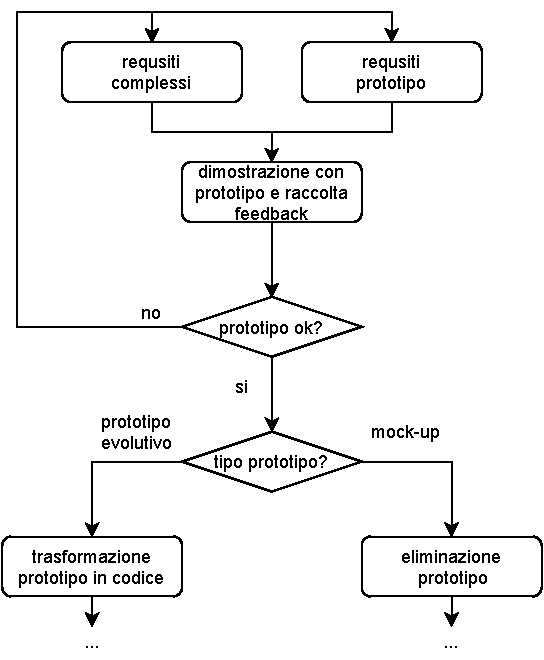
\includegraphics[scale = 0.8]{img/re4.pdf}
  \caption{Rappresentazione del processo tramite prototipi}
\end{figure}
Si ha anche il \textbf{knowledge reuse}, per velocizzare l'elicitation, riusando
conoscenze pregresse da sistemi simili a quello sotto studio.\\
Si hanno 3 fasi:
\begin{enumerate}
  \item trarre conoscenze e informazioni rilevanti da altri sistemi
  \item trasporle nel sistema in studio
  \item convalidare il risultato, adattarlo se necessario e integrarlo con la
  conoscenza del sistema già acquisita
\end{enumerate}
Tali conoscenze possono essere dipendenti o indipendenti dal dominio.\\
Si hanno i seguenti pro:
\begin{itemize}
  \item analisti esperti riutilizzano naturalmente dall'esperienza passata
  \item riduzione degli sforzi di eliciation
  \item ereditarietà della struttura e qualità delle specifiche del dominio
  astratto 
  \item efficace per completare i requisiti con aspetti trascurati
\end{itemize}
e i seguenti contro:
\begin{itemize}
  \item efficace solo se il dominio astratto è sufficientemente simile e
  accurato 
  \item definire domini astratti per una riusabilità significativa è difficile 
  \item si hanno forti sforzi di convalida e integrazione 
  \item le corrispondenze vicine possono richiedere adattamenti complicati
\end{itemize}
\textbf{Approfondimento su slide.}\\
Un'altra tecnica \textbf{artefact-driven} è il \textbf{card sort}, che consiste
nel chiedere agli 
stakeholder di suddividere un set di carte dove:
\begin{itemize}
  \item ogni carta cattura un concetto in modo testuale o grafico 
  \item carte raggruppate in sottoinsiemi in base ai criteri degli stakeholder 
\end{itemize}
L'obiettivo è acquisire ulteriori informazioni sui concetti già evocati. Per ogni
sottoinsieme, chiedere la proprietà condivisa implicita utilizzata per il
raggruppamento per poi ripetere con le stesse carte per nuovi raggruppamenti /
proprietà.
\paragraph{Stakeholders-driven}
Passiamo quindi alle tecniche in cui interagisce direttamente lo stakeholder,
senza la mediazione di artefatti.\\
La prima tecnica è l'\textbf{intervista} che consiste in:
\begin{itemize}
  \item selezione mirata dello stakeholder, in base alle informazioni necessarie
  \item fare l'intervista registrando le risposte
  \item scrivere il \textit{transcript} dell'intervista e produrre subito il
  report
  \item sottomettere all'intervistato il report per validazione
\end{itemize}
Si può avere un'intervista anche con più stakeholder (perdendo però in parte la
costruzione del rapporto personale con lo stakeholder). L'intervista è una
tecnica costosa e le interviste possono essere poche, bisogna quindi procedere
in modo attento.\\
Si hanno due tipi:
\begin{enumerate}
  \item \textbf{interviste strutturate}, dove si parte con un insieme di domande
  già scelto per un certo obiettivo. Si da poco spazio ad una discussione aperta
  \item \textbf{interviste non strutturate}, dove si da spazio alla discussione
  aperta e libera sul \textit{system-as-is}, sulle problematiche e sulle
  soluzioni. 
\end{enumerate}
Spesso si hanno interviste miste, nella prima parte strutturate e poi con
domande e argomenti liberi. Gli argomenti vanno calibrati così come il numero di
domande, per evitare perdite di tempo e di attenzione da parte dello
stakeholder.\\
Vediamo quindi qualche linea guida per la preparazione delle interviste.
\begin{itemize}
  \item bisogna arrivare preparati, tramite il background study
  \item per costruire un rapporto con lo stakeholder le domande devono essere su
  misura dello stesso, in base al suo lavoro e ruolo
  \item mettere in centro all'intervista necessità e problematiche
  dell'intervistato, chiarendo di essere interessati al suo punto di vista
  \item evitare che la discussioni dilaghi su argomenti inutili
  \item fare in modo che l'intervistato si senta a suo agio, magari iniziando
  con qualche chiacchiera informale e domande semplici per poi spostarsi su
  domande difficili
  \item dimostrarsi affidabile
  \item chiedere sempre ``perché'' cercando il rationale di ciò che si chiede
  \item evitare domande bias che influenzino la risposta
  \item evitare domande ovvie che facciano pensare all'intervistato che stia
  perdendo tempo
  \item evitare domande a cui sicuramente l'intervistato non sa rispondere
\end{itemize}
Nel transcript bisogna includere reazioni personali (anche se queste parti
possono essere tolte dalla copia di validazione).\\
Si hanno altri modi per interagire con lo stakeholder.\\
Talvolta si ha bisogno anche di altre modalità oltre la sola intervista.\\
Spesso è più facile infatti far osservare che descrivere a parole e quindi si
hanno \textbf{studi osservazionali ed etnografici}, ovvero studi che si basano
sull'osservazione degli stakeholders stessi all'azione, nell'ottica del
\textit{system-as-is}, osservando come svolgono vari task per cogliere problemi
e funzionalità. Si hanno due modalità di osservazione:
\begin{enumerate}
  \item \textbf{osservazione passiva}, dove non si produce interferenza sulle
  azioni dello stakeholder, guardando da fuori, registrando record e producendo
  un transcript. Si hanno due particolari \textbf{osservazioni passive}:
  \begin{enumerate}
    \item \textbf{protocol analysis}, dove si studia qualcuno che svolge un
    certo protocollo, un certo task (la slide dice spiegando contemporaneamente)
    \item \textbf{ethnographic studies}, studio che si svolge in un lungo
    periodo di tempo, dove si prova a scoprire le proprietà emergenti del gruppo
    sociale coinvolto
  \end{enumerate}
  \item \textbf{osservazione attiva}, dove si svolge in prima persona i task,
  diventando eventualmente team member, capendo attivamente come deve essere
  svolto un task
\end{enumerate}
Gli studi osservazionali aiutano a scoprire requisti che restano altrimenti
taciti e a scoprire problemi nascosti, che non si noterebbero
nell'intervista. Aiuta anche a contestualizzare le informazioni. È comunque
un'operazione lenta e costosa, dovendo recarsi di persona ad osservare ed
annotare. Può essere potenzialmente inaccurato in quanto una persona conscia di
essere osservata potrebbe comportarsi in modo diverso dallo
standard. L'osservazione si focalizza comunque solo sul \textit{system-as-is} e
non aiuta molto nel \textit{system-to-be}.\\
Si hanno altri modi di interazione con gli stakeholders tra cui le \textbf{group
sessions}, ovvero una famiglia di tecniche utili per la risoluzione di
conflitti. L'elicitation prende la forma di un ``workshop'' di uno o più giorni
in cui si ha una discussione tra vari partecipanti scelti in modo oculato a
seconda dall'obiettivo, innescando una discussione utile a comprendere il
\textit{system-to-be}. Mettendo insieme le parti con visioni conflittuali si
possono risolvere conflitti. Su hanno due tipologie di \textit{group sessions}:
\begin{enumerate}
  \item \textbf{strutturate} dove ogni partecipante ha un ruolo chiaramente
  definito: leader, moderatore, manager, utente, sviluppatore, etc$\ldots$
  Ognuno contribuisce in funzione del ruolo, permettendo di ragionare su
  requisiti di più alto livello, comuni a più figure, e su conflitti ad alto
  livello 
  \item \textbf{non strutturate}, dette anche \textbf{sessioni brainstorming},
  dove i partecipanti non hanno un ruolo definito. La sessione è formata da due
  fasi:
  \begin{enumerate}
    \item \textbf{generazione delle idee}, dove tutti espongono le proprie idee
    in merito al problema/conflitto che ha generato la sessione
    \item \textbf{valutazione delle idee}, dove tutte le idee vengono
    analizzate una per una e valutate per valore, costo, fattibilità etc$\ldots$
    in modo da arrivare una visione condivisa sugli approcci da usare secondo
    una certa prioritizzazione
  \end{enumerate}
\end{enumerate}
Si ha il pro di poter esplorare varie opzioni e a portare a risoluzioni
sfruttando anche l'inventiva dei partecipanti. La composizione del gruppo è
comunque critica, molti potrebbero non avere tempo, alcuni potrebbero prendere
posizioni dominanti introducendo bias, condizionando la discussione e le
decisioni. Si rischia inoltre che la discussione diverga verso inutilità senza
convergere sugli aspetti per cui è stata convocata la sessione.\\
\textbf{Ogni attività, sia artefact-driven che stakeholder-driven viene svolta
  solo se si hanno chiari gli obiettivi che si vogliono ottenere con tale
  attività.}
\newpage
\subsection{Evaluation \& agreement}
\subsubsection{Requirements Evaluation}
In questa fase si studia:
\begin{itemize}
  \item \textit{inconsistency management}, in ottica di:
  \begin{itemize}
    \item tipi di inconsistenza
    \item manipolazione delle stesse 
    \item gestione dei conflitti in modo sistematico
  \end{itemize}
  \item la valutazione di alternative per prendere decisioni
  \item la prioritizzazione dei requisti, \textit{requirements prioritization}
\end{itemize}
\paragraph{Consistency management}
\begin{definizione}
  Definiamo \textbf{inconsistenza} come la violazione della regola di coerenza
  tra gli elementi.
\end{definizione}
Si hanno due tipi:
\begin{enumerate}
  \item \textbf{inter-viepoint}, quando ogni stakeholder ha il suo focus e il
  suo punto di vista
  \item \textbf{intra-viewpoint}, quando si hanno conflitti tra i requisti di
  qualità (conflitti per esempio tra sicurezza e accessibilità)
\end{enumerate}
A livello di tempo le inconsistenze vanno identificate e risolte:
\begin{itemize}
  \item \textit{non troppo presto}, per avere prima un'elicitation più
  approfondita 
  \item \textit{non troppo tardi}, per permettere lo sviluppo del software
\end{itemize}
Dal punto di vista dei tipi di inconsistenza abbiamo:
\begin{itemize}
  \item \textbf{terminology clash}, avendo lo stesso concetto denominato
  diversamente in statement diversi
  \item \textbf{designation clash}, avendo lo stesso nome per concetti diversi
  in statement diversi
  \item \textbf{structure clash}, avendo lo stesso stesso concetto strutturato
  in modo diverso in statement diversi
\end{itemize}
Distinguiamo inoltre:
\begin{itemize}
  \item \textbf{conflitto forte}, avendo statement non soddisfacibili
  contemporaneamente (ad esempio $S\land \neg S$)
  \item \textbf{conflitto debole (\textit{divergenza})}, avendo statement non
  soddisfacibili contemporaneamente in certe condizioni e con certi vincoli
\end{itemize}
Per gestire i clash (scontri) in termini di terminologia, design e/o struttura
si usa il glossario costruito nella fase di elicitation (dove vengono anche
usati eventualmente acronimi).\\
Gestire le inconsistenze è difficoltoso a causa:
\begin{itemize}
  \item obiettivi personali in conflitto da parte degli stakeholder (cosa che
  andrebbe gestita alla base propagandone i risultati al livello dei
  requirements)
  \item legati ad ambiti non funzionali, come ad esempio prestazioni vs
  sicurezza, confidenzialità vs consapevolezza, etc$\ldots$ (cosa che andrebbe
  gestita tramite uno studio dei tradeoff, i compromessi, migliori) 
\end{itemize}
Come detto la gestione dei conflitti avviene in modo schematico, tramite il
seguente schema:
\begin{figure}[H]
  \centering
  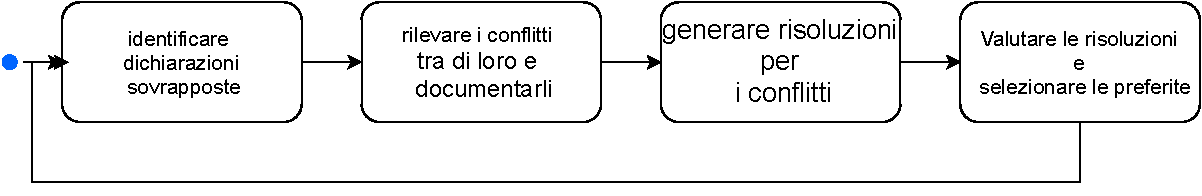
\includegraphics[scale = 0.6]{img/re5.pdf}
\end{figure}
Nel dettaglio:
\begin{itemize}
  \item per la prima fase con sovrapposizione/overlap indichiamo il riferimento
  a termini o fenomeni comuni 
  \item per la seconda il riconoscimento può essere fatto informalmente, tramite
  euristiche sulle categorie dei requisiti in conflitto, o
  formalmente. Il riconoscimento deve essere documentato per una successiva
  risoluzione e analisi dell'impatto. Si usano strumenti come
  l'\textbf{interaction matrix} che presenta su righe e colonne gli statement e
  negli incroci indica:
  \begin{itemize}
    \item 1 per il conflitto
    \item 0 per nessun overlap
    \item 1000 per overlap senza conflitto
  \end{itemize}
  Avendo, per ogni statement $S_i$, indicando con $S_i$ la riga/colonna
  corrispondente (sono uguali):
  \[conflict(S_i)= \left(\sum_{s\in S_i}s\right) \mod 1000\] 
  \[nonConflictingOverlaps(S_i)= \Bigl\lfloor{\sum_{s\in
        S_i}}{1000}\Bigr\rfloor\]
  \begin{esempio}
    \begin{table}[H]
      \centering
      \begin{tabular}{c||c|c|c|c|c}
        statement & $S_1$ & $S_2$ & $S_3$& $S_4$ & total\\
        \hline
        $S_1$ & 0 & 1000 & 1 & 1 & 1002\\
        $S_2$ & 1000 & 0 & 0 & 0 & 1002\\
        $S_3$ & 1 & 0 & 1 & 1 & 1002\\
        $S_4$ & 1 & 0 & 1 & 0 & 1002\\
        total & 1002 & 1000 & 2 & 2 & 1002\\
      \end{tabular}
    \end{table}
    \[conflict(S_1)=2\]
    \[nonConflictingOverlaps(S_2)=1\]
  \end{esempio}
 
  \item per la terza fase è meglio:
  \begin{itemize}
    \item esplorare prima più risoluzioni, generate tramite tecniche di
    elicitation e usando tattiche di risoluzione dei conflitti:
    \begin{itemize}
      \item evitare condizioni a contorno
      \item ripristinare statement in conflitto
      \item indebolire gli statement in conflitto
      \item non considerare statement a bassa priorità
      \item approfondire source e target del conflitto
    \end{itemize}
    \item confrontare, selezionare e concordare il preferito poi
  \end{itemize}
  Si trasformano quindi statement in conflitto (e parti coinvolte) in nuovi
  requisiti 
  \item per la quarta fase si usano vari criteri per la scelta:
  \begin{itemize}
    \item ontributo a requisiti non funzionali critici 
    \item contributo alla risoluzione di altri conflitti e rischi 
    \item applicazione dei principi di \textit{risk analysis}
  \end{itemize}
\end{itemize}
\paragraph{Requirements prioritization}
Ai vari requisti va imposta una prioritizzazione, per vari scopi:
\begin{itemize}
  \item risoluzione dei conflitti 
  \item limitazioni delle risorse (budget, personale, programmi) 
  \item sviluppo incrementale 
  \item ripianificazione a causa di problemi imprevisti
\end{itemize}
e si hanno vari principi per una buona riuscita della stessa, che può essere
svolta: 
\begin{enumerate}
  \item tramite livelli ordinati di uguale priorità, in un piccolo numero 
  \item tramite livelli relativi ("maggiore di" etc$\ldots$) 
  \item tramite requisiti comparabili: stessa granularità, stesso livello di
  astrazione  
  \item tramite requisiti non mutuamente dipendenti (uno può essere mantenuto,
  un altro eliminato) 
  \item tramite un'accordo con i vari partecipanti e stakeholder
\end{enumerate}
Per i primi tre posso usare una tecnica sistematica basata su diversi step:
\begin{itemize}
  \item stimare il contributo relativo di ogni richiesta al \textbf{valore} del
  progetto 
  \item stimare il contributo relativo di ciascuna richiesta al \textbf{costo}
  del progetto 
  \item tracciare il \textbf{diagramma valore-costo}
\end{itemize}
\begin{figure}
  \centering
  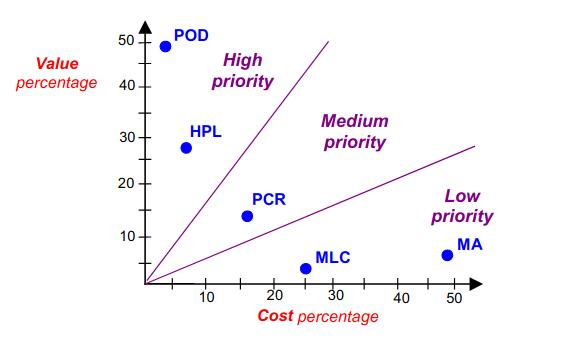
\includegraphics[scale = 0.6]{img/re6.jpg}
  \caption{Grafico costo-valore con 5 requisti d'esempio:
    POD:  Produce Optimal meeting Dates,
    HPL: Handle Preferred Locations,
    PCR: Parameterize Conflict Resolution,
    MLC: Support Multi-Lingual Communication e
    MA:  Provide Meeting Assistant}
\end{figure}
Si usa quindi la tecnica AHP dalla \textbf{Decision Theory} dove si cerca di
capire in che proporzione ogni requisito $R_i$ contribuisce al criterio $crit$,
che sarà prima il \textbf{valore}, $crit=value$, e poi il \textbf{costo},
$crit=cost$.\\
Si hanno quindi due step:
\begin{enumerate}
  \item si usa la \textbf{comparison matrix} stimando i contributi di ogni
  requisito sul criterio da studiare.\\
  Avendo $N$ requisiti:
  \[R_{ij}=\frac{1}{R_{ij}}\mbox{ se } 1\leq i,j\leq N\]
  \begin{esempio}
    \textit{(i conti potrebbero essere errati)}
    \begin{table}[H]
      \centering
      \begin{tabular}{c||c|c|c|c|c}
        crit=value & $R_1$ & $R_2$& $R_3$ & $R_4$ & $R_5$\\
        \hline
        $R_1$ &1 & 3 & 5 & 9 & 7\\
        $R_2$ & $\frac{1}{3}$ & 1 & 3 & 7 & 7\\
        $R_3$ & $\frac{1}{5}$ & $\frac{1}{3}$ & 1 & 5 & 3\\
        $R_4$ & $\frac{1}{9}$ & $\frac{1}{7}$ & $\frac{1}{5}$ & 1 &$\frac{1}{3}$\\
        $R_5$ &  $\frac{1}{7}$ & $\frac{1}{7}$ & $\frac{1}{3}$ & 3 & 1
      \end{tabular}
    \end{table}
  \end{esempio}
  \item si determina quanto questo si distribuisce
  tra tutti i requisti, tramite gli \textbf{autovalori} della matrice.\\
  Inoltre le colonne vengono normalizzate tramite:
  \[R_{ij}=\frac{R_{ij}}{\sum_i R_{ij}}\]
  \newpage
  e aggiungendo la media sulle righe per valutare il contributo del requisito
  sul criterio:
  \begin{esempio}
    \textit{(i conti potrebbero essere errati)}
    \begin{table}[H]
      \centering
      \begin{tabular}{c||c|c|c|c|c||c}
        & $R_1$ & $R_2$& $R_3$ & $R_4$ & $R_5$ & contributo\\
        \hline
        $R_1$ & 0.56 & 0.65 & 0.52 & 0.36 & 0.38 & 0.49\\
        $R_2$ & 0.19 & 0.22 & 0.31 & 0.28 & 0.38 & 0.28\\
        $R_3$ & 0.11 & 0.07 & 0.10 & 0.20 & 0.16 & 0.13\\
        $R_4$ & 0.06 & 0.03 & 0.02 & 0.04 & 0.02 & 0.03\\
        $R_5$ & 0.08 & 0.03 & 0.03 & 0.12 & 0.05 & 0.07
      \end{tabular}
    \end{table}
  \end{esempio}
\end{enumerate}
AHP permette di assicurare stime e rapporti consistenti.
\subsection{Specification \& documentation}
Parliamo quindi della fase di \textbf{specification \& documentation}.\\
In questa fase si documentano in modo preciso i requisiti scoperti. Si
descrivono in modo preciso le feature e i concetti rilevanti per il
progetto. Nel dettaglio si definiscono in modo preciso:
\begin{itemize}
  \item obiettivi, concetti, proprietà di dominio rilevanti, requisiti di
  sistema/software, ipotesi, responsabilità 
  \item il rationale delle opzioni scelte
  \item un'indicazione sulle varianti e sulle evoluzioni previste
\end{itemize}
Il documento deve avere una struttura coerente. Tale documento è detto
\textbf{requirements Document (\textit{RD})}. Qualora i requisti siano stati
messi online si procede alla costruzione di un db che tiene traccia dei
requisti. In ogni caso il contenuto deve essere accessibile e comprensibile da
tutte le parti interessate, aggiungendo spesso in allegato anche costi, workplan
e piani di delivery. Bisogna capire come effettivamente documentare i
requisiti.\\
La prima opzione è l'utilizzo del linguaggio naturale in modo
svincolato, in prosa. Si ha una forte espressività ma, in assenza di regole
sulla scrittura si rischia di produrre una sorta di romanzo, producendo qualcosa
di poco gestibile. Il linguaggio naturale inoltre può nascondere ambiguità
(basti pensare anche solo a sequenze di \textit{or} e \textit{and} in assenza di
uno schema logico fisso). Usando il linguaggio naturale privo di vincoli si
hanno quindi rischi ma si può usare un \textit{linguaggio naturale
  strutturato}. Si introducono quindi due tipi di regole:
\begin{enumerate}
  \item \textbf{local rules}, che riguardano la scrittura del singolo requisito
  \item \textbf{global rules}, che riguardano le regole sulla scrittura
  dell'intero documento e sull'insieme dei requisti
\end{enumerate}
Abbiamo però, in primis, alcune regole stilistiche generali (le stesse che si
dovrebbero applicare anche per una tesi):
\begin{itemize}
  \item scrivere pensando a chi deve leggere, che deve essere ben identificato
  \item spiegare cosa stiamo per scrivere prima di specificarlo nel dettaglio
  \item prima motivare le scelte, indicare le scelte e poi fare un sommario
  delle stesse 
  \item assicurarsi che ogni concetto usato nei requisiti sia stato prima ben
  definito 
  \item chiedersi se quanto scritto è comprensibile e rilevante (per capirlo
  basta cancellare quanto scritto e vedere se si capisce ancora)
  \item per ogni frase/elemento del documento indicare uno e un solo requisito o
  assunzione o proprietà di dominio, evitando di mischiare troppe cose
  \item scrivere frasi brevi
  \item distinguere ciò che è obbligatorio da ciò che è desiderabile
  \item evitare acronimi non necessari ed evitare l'abuso del gergo informatico
  \item usare esempi esplicativi
  \item usare diagrammi o illustrazioni quando utile
\end{itemize}
In termini di local rules si hanno dei template per scrivere i requisiti, usando
anche un solo standard per tutti i requisti. Un esempio di template potrebbe
contenere:
\begin{itemize}
  \item identificatore del requisito (con uno schema di naming significativo,
  magari con uno schema gerarchico con combinazioni di caratteri tramite
  separatore per specificare al meglio il requisito)
  \item categoria del requisito (funzionale, assunzione etc$\ldots$)
  \item specifica del requisito (usando le regole stilistiche)
  \item criterio di fit (una sorta di test di accettazione, usato quindi per
  quantità/concetti misurabili, essendo critico quindi per requisiti non
  funzionali) 
  \item fonti di elicitazione
  \item rationale
  \item interazioni con altri requisti (contribuzioni, dipendenze e conflitti)
  \item livello di priorità
  \item livelli di stabilità (per indicare le chance di cambiamenti)
\end{itemize}
Per le global rules si ha una forma standard data da \textbf{IEEE std-830}, il
più diffuso. Si hanno varie macrocategorie a loro volta suddivise:
\begin{enumerate}
  \item introduzione (dove si specifica anche quale parte del documento
  interessi ai vari stakeholder)
  \begin{enumerate}
    \item motivazioni del documento
    \item scopo del prodotto
    \item definizioni, acronimi, sigle e abbreviazioni
    \item reference, fonti di elicitazione
    \item overview dell'organizzazione del documento
  \end{enumerate}
  \item descrizione generale
  \begin{enumerate}
    \item prospettive del prodotto
    \item funzionalità principali
    \item caratterizzazione degli utenti
    \item vincoli generali sull'ambiente (che non possono esse modificati ma con
    i quali si deve integrare il prodotto)
    \item assunzioni sul prodotto e dipendenze del prodotto
    \item ripartizione dei requisti
  \end{enumerate}
  \item requisiti specifici (spesso per i dev), usando magari il template visto
  prima. Si hanno quindi varie categorie di requisiti che articolano le varie
  sezioni del capitolo:
  \begin{enumerate}
    \item requisiti funzionali (che a sia volta un'organizzazione interna in
    base a vari fattori, come aree funzionali, componenti etc$\ldots$)
    \item Requisiti per l'interfaccia esterna
    \item requisiti per le prestazioni
    \item vincoli di progettazione
    \item attributi di qualità del software
    \item altri requisiti
  \end{enumerate}
  \item appendice
  \item indice
\end{enumerate}
Una variante p il \textbf{template VOLERE} dove si hanno sezioni esplicite per
proprietà del dominio, costi, rischi, piano di lavoro di sviluppo etc$\ldots$\\
Si hanno anche opzioni aggiuntive oltre al linguaggio naturale. In primis si ha
l'uso di diagrammi, con quindi una \textbf{notazione semi-formale}, in quanto si
ha una sintassi formale essendo i vari diagrammi formalmente definiti ma
interpretazione degli stessi può comunque ssere ambigua.\\
I diagrammi sono utili per complementare quanto scritto in linguaggio naturale,
che risulta spesso troppo complesso e articolato. Un diagramma può semplificare
quanto scritto e rappresentare il tutto in modo compatto. L'uso di diagrammi
permette di comunicare più semplicemente e viene usato per aspetti specifici del
sistema. Si ha comunque la stessa ambiguità di interpretazione che si aveva nei
linguaggi naturali. vediamo alcuni diagrammi.\\
Un primo esempio è il \textbf{problem diagram} che descrive i requisiti a livello
di sistema. Si mostrano le componenti del sistema dove ogni componente è
indicato tramite un rettangolo con doppia linea a sinistra. Il sistema comunica
con diversi elementi dell'ambiente, indicati da rettangoli. Si può specificare
testualmente un requisito e riferirlo agli elementi dell'ambiente citati nel
requisito, che è posto in un ellisse tratteggiato. Posso avere riferimenti e
vincoli sugli elementi a partire dal requisito. Tutte le interazioni sono
decorate con gli eventi che sono rilevanti per l'interazione con il produttore
dell'evento indicato tramite le maiuscole e il nome dell'evento, a loro volta
separati da ``!''. Con questo tipo di diagramma si cattura il contesto del
requisito, legandolo  componenti dell'ambiente e componenti del sistema, tramite
specifici eventi. Si identificano a colpo d'occhio gli elementi rilevanti per un
certo requisito.
Esempio di problem diagram nella figura \ref{fig:pd}.
\begin{figure}
  \centering
  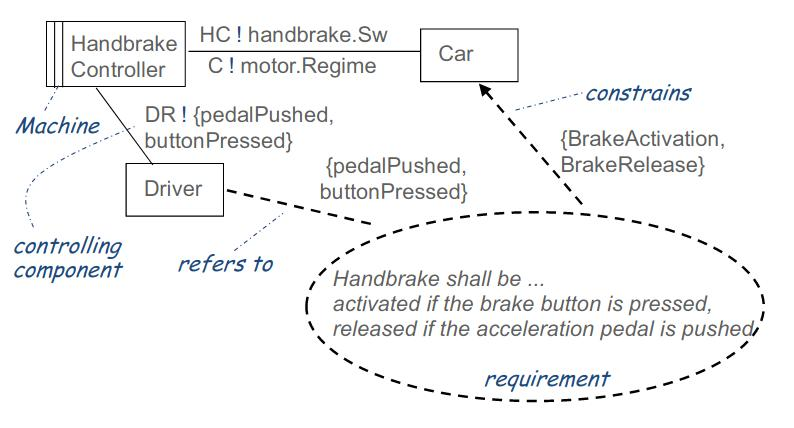
\includegraphics[scale = 0.4]{img/pd.jpg}
  \caption{Esempio di problem diagram}
  \label{fig:pd}
\end{figure}
Questa rappresentazione può prendere la forma di veri e propri pattern detti
\textbf{problem pattern} per semplificare la rappresentazione. Si ottengono i
frame diagrams, che hanno la stessa rappresentazione dei problem diagram con la
differenza che si ha qualche informazione in più:
\begin{itemize}
  \item tipo di componente (indicato con un quadratino in basso a destra nel
  rettangolo della componente) specificato da una lettera:
  \begin{itemize}
    \item C: causal, causa-effetto
    \item B: biddable, non predicibile
    \item X: lexical, lessicale, specifica artefatti
  \end{itemize}
  \item tipo di evento (posto) dopo il ``!'' sopra descritto) specificato da una
  lettera: 
  \begin{itemize}
    \item C: causal, diretta conseguenza di altri eventi
    \item E: event, che non sono diretta conseguenza ma che sono prodotti in modo
    spontaneo 
    \item X: lexical, dati che vengono utilizzati per produrre qualcosa
  \end{itemize}
\end{itemize}
Tali pattern vengono istanziati nei vari casi specifici (esempio completo nelle
slide). Si ha un catalogo di tali pattern caricato sulla pagina del corso.\\
Un altro diagramma tipico è quello ER per specificare entità che entrano in
gioco in certi aspetti dei requisiti, specificandole in modo schematico. Si
usano anche diagrammi di dominio, di classe etc$\ldots$, non descrivendo più
comportamenti ma strutture, domini etc$\ldots$\\
Tipi di diagramma invece da approfondire sono i \textbf{SADT diagrams} che si
dividono in due tipi e permettono di specificare il comportamento di alcune
attività scomponendolo e aggiungendo varie informazioni.
\begin{enumerate}
  \item actigram, di tipo activity-driven, si concentra sulle attività e mostra
  le dipendenze tra attività in termini di dati. Le attività sono indicate
  dentro rettangoli e si hanno una serie di frecce che a seconda della direzione
  variano il significato:
  \begin{itemize}
    \item $\longrightarrow$ per l'input di dati
    \item $\longleftarrow$ per l'output di dati
    \item $\downarrow$ per il data/event controlling, ovvero dati o eventi che
    controllano il comportamento dell'attività, sono magari aspetti di
    configurazione etc$\ldots$ che influenzano l'attività
    \item $\uparrow$ per l'unità che processerà l'attività (opzionale)
  \end{itemize}
  \begin{figure}
    \centering
    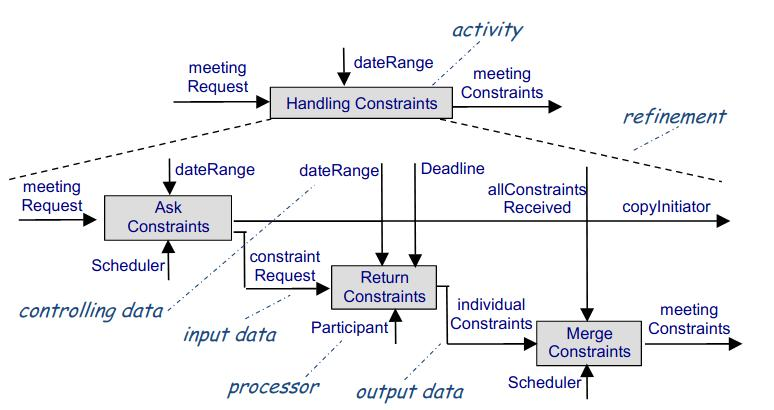
\includegraphics[scale = 0.5]{img/agram.jpg}
    \caption{Esempio di actigram con sotto un raffinamento della parte
      superiore} 
    \label{fig:agram}
  \end{figure}
  Vedere figura \ref{fig:agram}.
  \item datagram, di tipo data-driven, si concentra sui dati e mostra
  le dipendenze tra dati in termini di attività. I dati sono indicate
  dentro rettangoli e si hanno una serie di frecce che a seconda della direzione
  variano il significato:
  \begin{itemize}
    \item $\longrightarrow$ per l'input di attività che producono il dato
    \item $\longleftarrow$ per l'output di attività verso le quali serve il dato
    \item $\downarrow$ per le attività di validazione del dato
    \item $\uparrow$ per le risorse necessarie a memorizzare e gestire il dato
  \end{itemize}
  
  \begin{figure}
    \centering
    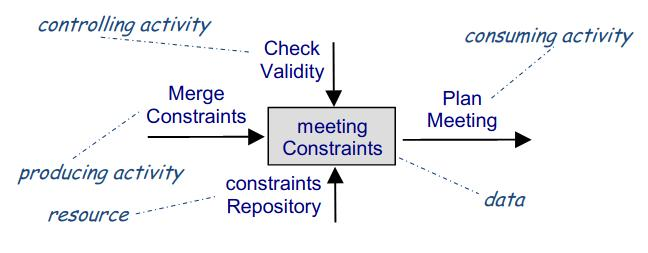
\includegraphics[scale = 0.5]{img/dgram.jpg}
    \caption{Esempio di datagram}
    \label{fig:dgram}
  \end{figure}
  Vedere figura \ref{fig:dgram}.
\end{enumerate}
La coerenza tra di due diagrammi è fondamentale avendo una rapporto di
\textbf{dualità} tra essi quindi i dati e le attività presenti in uno devono
apparire anche nell'altro.

Questo strumenti si prestano a documentare workflow molto semplici. In ogni
caso:
\begin{itemize}
  \item gni attività deve avere un input e un output 
  \item tutti i dati devono avere un produttore e un consumatore 
  \item i dati I/O di un'attività devono apparire come dati I/O delle
  sottoattività 
  \item ogni attività in un datagramm deve essere definita in un actigramma
\end{itemize}
Un altro diagramma classico è il \textbf{case use diagram} per
visualizzare i requisiti identificati, che prendono forma di casi d'uso con gli
attori che partecipano allo svolgimento dei requisiti. Si hanno le varie
relazioni di inclusione etc$\ldots$\\
Un altro strumento utile nella definizione di workflow è l'\textbf{eventi trace
  diagrams}, ovvero i diagrammi di sequenza. Se ne hanno vari tipi con sintassi
più o meno ricche ma in generale si hanno $N$ elementi che partecipano
all'esecuzione che viene mostrata visualmente tramite richieste e risposte,
sincrone o meno, che vengono indicate cronologicamente dall'alto al
basso. Questa visualizzazione compatta aiuta nel momento in cui il linguaggio
naturale diventa troppo complesso e verboso per spiegare una certa sequenza di
azioni. \\
Un altro diagramma usato è il \textbf{state machine diagram} per mostrare in
quali stati un particolare elemento si trova e quali transizioni/eventi
modificano i suoi stati. Questi diagrammi sono utili in quanto in modo compatto
rappresenta il ciclo di vita di una certa componente, facilitando la creazione
del sistema. \\
Come altro diagramma abbiamo il \textbf{R-net diagram} che permette di mostrare
come reagisce un sistema in base ad un certo stimolo. È quindi un albero che
parte con uno stimolo, dopo il begin, posto in un esagono e si sviluppo in base
alle varie alternative in corrispondenza di punti di decisione (indicati come
pallini). Nei rettangoli si hanno le azioni che sono svolte in conseguenza allo
stimolo. Un esempio si ha in figura \ref{fig:rnet}.
\begin{figure}
  \centering
  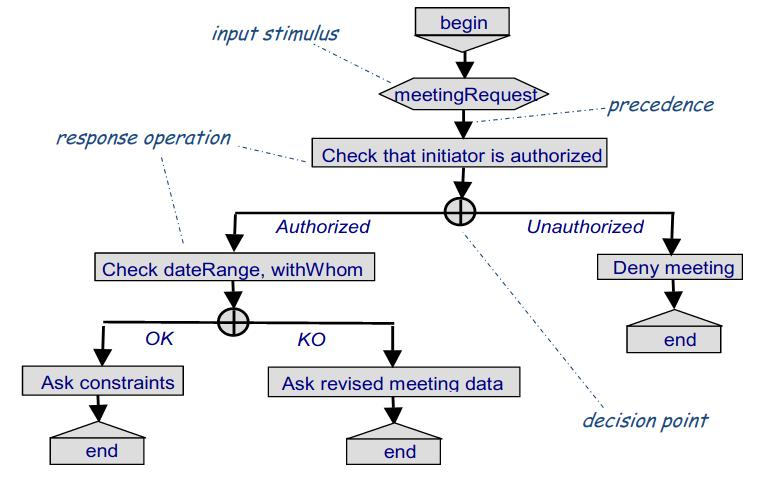
\includegraphics[scale = 0.5]{img/rnet.jpg}
  \caption{Esempio di R-net diagram}
  \label{fig:rnet}
\end{figure}
I diagrammi sono tra loro complementari ma hanno anche delle intersezioni tra
loro e anche con il testo e tutto deve comunque restare coerente. Si rischia di
introdurre inconsistenze. Si hanno alcune regole di consistenza per i diagrammi
che vengono usate da diversi strumenti per verificare la consistenza tra i vari
diagrammi. \\
A questo punto è doveroso citare uno degli standard per la modellazione di
diagrammi: \textbf{Unified Modeling Language (\textit{UML})}. Al suo interno si
hanno, con regole di coerenza tra essi:
\begin{itemize}
  \item class diagrams
  \item use case diagrams
  \item sequence diagrams
  \item state diagrams
\end{itemize}
In conclusione i diagrammi hanno il pro di essere in grado di dare una buona
panoramica e struttura/comportamento, facile da trasmettere e comprendere, di
aspetti importanti. Sono inoltre supportati da vari tool di analisi. Il contro è
sempre la specifica ambigua semi-formale che può anche limitare l'analisi degli
stessi. Inoltre si concentrano solo su aspetti funzionali e strutturali.
Si hanno anche gli \textbf{statechart} (figura \ref{fig:sta}) per la descrizione
di sistemi paralleli 
che usano la semantica interleaving ovvero per 2 transizioni che si attivano
nello stesso stato, una viene presa dopo l'altra, in modo non deterministico.
\begin{figure}
  \centering
  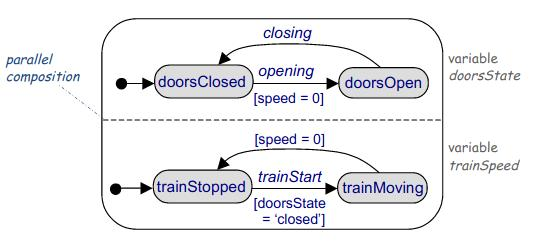
\includegraphics[scale = 0.5]{img/sta.jpg}
  \caption{Esempio di R-net diagram}
  \label{fig:sta}
\end{figure}
Si ha
quindi in generale la necessità di una semantica formale per aspetti
\textit{mission-critical} e la cosa non viene garantita dai diagrammi ma si
hanno linguaggi apposta (e diagrammi apposta) la cui
creazione/gestione/documentazione è assai costosa per cui vengono usati solo in
casi estremamente specifici. Approfondiamo quindi questi linguaggi e questa
notazione. \\
Si parla sia di sintassi che di semantica. Tali definizioni formali permettono
che il compilatore sia in grado di processare tali specifiche. Si ha quindi un
livello di precisione alto e non si ha ambiguità, permettendo analisi di
consistenza e coerenza delle specifiche (fatta direttamente dal
calcolatore). Una sintassi/semantica formale è quella data dalla logica
proposizionale e dalle \textbf{formule ben formate}. Si ha quindi un linguaggio
basato sui connettori logici e sulle regole per avere formule ben formate. Ogni
statement può quindi essere interpretato con il valore di verità con le regole
definite dalla logica e dalle tabelle di verità (ovviamente può farlo il
calcolatore). Si vede quanto produrre tutto questo per un progetto enorme
risulti costoso. Vengono quindi usate le classiche regole di inferenza. Si usa
anche la \textbf{logica predicativa del primo ordine}.\\
Un altro strumento usato è la \textbf{logica temporale} con l'aggiunta dei
connettivi temporali.\\
Si ha un approccio formale anche su specifiche state-based dove si specifica in
modo formale cosa sia l'insieme degli stati che il sistema può attraversare e
come delle operazioni modificano lo stato. Si usano linguaggi come $Z$ basati
sulla teoria degli insiemi. Ogni stato è caratterizzato da pre e post condizioni
e si studiano le regole in termini di invarianti che lo stato deve
soddisfare. Con $Z$ si producono schemi come:
\begin{figure}[H]
  \centering
  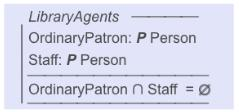
\includegraphics[scale = 0.6]{img/z.jpg}
\end{figure}
dove si specifica un certo elemento, gli attributi di stato con $P$ che indica
l'\textit{insieme delle parti} che precede il tipo. Si ha poi un invariante per
gli attributi che definisce l'elemento. Si ha quindi una caratterizzazione
basata sulla teoria degli insiemi. Si hanno sia tipi primitivi che
strutturati. Per definire invece le modifiche che portano a nuovi stati, ovvero
per definire le operazioni si usa una simile sintassi:
\begin{figure}[H]
  \centering
  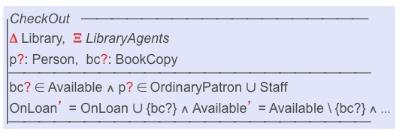
\includegraphics[scale = 0.6]{img/z2.jpg}
\end{figure}
Sopra si hanno tutti gli elementi coinvolti nell'operazione. La prima linea
della parte sotto è per le precondizioni, quella sotto per le postcondizioni,
entrambe con la notazione insiemistica. Gli elementi sono inoltre
così decorati: 
\begin{itemize}
  \item \texttt{stateVar?:Type} indica una variabile di input
  \item \texttt{stateVar':Type} indica una variabile di output mutevoli (?)
  \item \texttt{stateVar!:Type} indica una variabile di output esterne e non
  mutevoli (?
  \item \texttt{$\Delta$ schema} indica che si ha una modifica delle variabili
  importate dallo schema
  \item \texttt{$\Xi$ schema} indica che non si ha una modifica delle variabili
  importate dallo schema
\end{itemize}
Il cambiamento di stati ben definito diventa studiabile e simulabile, studiando
lo spazio di comportamenti del sistema a questo livello di astrazione,
individuando problemi che porterebbero alla correzione di requisiti.
Si può avere anche l'inclusione di più schemi. Con questa specifica state-based
si hanno vari pro:
\begin{itemize}
  \item automazione semplice grazie a logica, matematica discreta, studio degli
  invarianti etc$\ldots$
  \item ottimi meccanismi di strutturazione per comporre unità e strutture stati
  complessi
  \item permette l'analisi automatica: type checking, consistency
  checking, etc$\ldots$
\end{itemize}
Di contro non permette di studiare altro se non aspetti funzionali e non ha
un'historical referencing (anche se si hanno vari workaround per l'encoding di
stati passati).\\
Si ha anche una \textbf{specifica algebrica} per formalizzare le leggi che
compongono le operazioni, viste come funzioni matematiche senza esplicita
nozione di stato. Si ha invece un system history avendo una ``traccia'' delle
operazioni. Si hanno tipi di dato astratti, parametrizzazione, equazioni
condizionali e funzioni parziali. Si hanno tre tipi di operazione
(\textit{capire bene questa cosa su slide}):
\begin{enumerate}
  \item modifiers, per produrre qualsiasi istanza di concetto mediante
  composizione con altri modifier 
  \item generators, ovvero un sottoinsieme minimo di modifiers per generare
  qualsiasi istanza di concetto con un numero minimo di composizioni 
  \item obsevers, per ottenere informazioni pertinenti su qualsiasi istanza di
  concetto
\end{enumerate}
\textbf{Spesso si hanno funzioni ricorsive.}\\
\textbf{Vari esempi su slide}.\\
Come vantaggi si hanno:
\begin{itemize}
  \item analisi automatica efficiente
  \item specifiche eseguibili
  \item ricchi meccanismi di strutturazione (import, ereditarietà etc$\ldots$)
\end{itemize}
Di contro si ha una limitata potenza espressiva (solo equazioni senza historical
referencing) e una forte vicinanza alla programmazione (comportando difficoltà 
di validazione in caso, ad esempio, di ricorsioni).\\
Tendenzialmente i limiti della notazione formale sono sempre questi (oltre alla
difficoltà di lettura/scrittura), anche se permette alta precisione, pochi
difetti di specifica, analisi sofisticata (anche automatica), generazione di
artefatti come test cases, codice etc$\ldots$.
Ricapitolando:
\begin{itemize}
  \item il linguaggio naturale ``puro'' non è un'opzione
  \item il linguaggio naturale strutturato è quello più usato
  \item i diagrammi sono un'ottima aggiunta al linguaggio naturale
  \item la notazione formale è usata in rare circostanze
\end{itemize}

\end{document}  
% LocalWords:  Machine Learning waterfall png img slides jpg testing self step
% LocalWords:  organizing continuous refactoring Scrum scrum product backlog as
% LocalWords:  items dev members owner definzione stakeholders planning daily
% LocalWords:  review retrospective Programming Extreme extreme programming one
% LocalWords:  stories Short Releases Metaphor Simple Pair Collective Ownership
% LocalWords:  Integration Customer Coding workspace collective ownership cloud
% LocalWords:  DevOps operation deployment Amazon Netflix Facebook Development
% LocalWords:  Monitoring primis monitoring tool Evangelist automation expert
% LocalWords:  Security Engineer Developer Quality Assurance deploy Centric and
% LocalWords:  Action Responsibility Improvement Automate everything Work Git
% LocalWords:  devops lifecycle Build version control repository commit update
% LocalWords:  branch develop merge ndo hotfix feature fix pipelines push gates
% LocalWords:  quality phase component subsystem system production unit static
% LocalWords:  analysis mocks stubs deployato integration security tests Ops VM
% LocalWords:  downtime unstable naive Incremental wrt users Dark launching VMs
% LocalWords:  Canary releases Experimentation requests Gradual upgrades Green
% LocalWords:  rollout upgrade Rolling replicas components with backups Rainbow
% LocalWords:  incremental back experimentation load balancer gradual rolling
% LocalWords:  upgradate green router ridireziona rollback rainbow bacward ftp
% LocalWords:  compatibility backward Deployable units virtual machine shell UI
% LocalWords:  containers l'hypervisor dall'hypervisor tenant engine app store
% LocalWords:  dell'hypervisor dell'hypervisor l'hypervisor dall'hypervisor ELK
% LocalWords:  device stack Elasticsearch Kibana Logstash log series dashboard
% LocalWords:  tools Svn Ecplipse build Ant Java Maven Gradle JUnit Jenkins err
% LocalWords:  Bamboo Ansible Pupper Saltstack SaltStack Relic Sensu Splunk cut
% LocalWords:  Nagios Risk risk risk exposure outcome unsatisfactory deadline
% LocalWords:  deadlines triggers risks process related assessment contingency
% LocalWords:  prioritizzazione identification prioritization resolution list
% LocalWords:  gold plating science brainstorming decision tree node errr RRL
% LocalWords:  derivation plottando scatterplot reduction leverage defect plan
% LocalWords:  detection prevention impact matrix combineReduction Capability
% LocalWords:  overallEffect Maturity CMMI Institute CMM best practices project
% LocalWords:  CMMs cmmi configuration required expected purpose statement work
% LocalWords:  introductory specific goals generic example subpractices level
% LocalWords:  elaborations capability levels maturity performed managed policy
% LocalWords:  defined initial quantitatively optimizing GG profile improvement
% LocalWords:  planned executed org PM Requirements requirements adaptive to is
% LocalWords:  cruise legacy cards db next descriptive statements prescriptive
% LocalWords:  shared fenomena error domain properties assumptions pdf Parnas
% LocalWords:  simil embedded firewall tracciabilità forward reference slide RD
% LocalWords:  understanding elicitation agreement rationale Document bias
% LocalWords:  stakeholder engagement transcript osservazionali Evaluation
% LocalWords:  interaction elicitazione
